\section{Implementation}

The system involves a series of core modules such as video shot detection, audio
processing and subtitle processing, which are shown in Figure \ref{fig:DesignOverview}.

The following section outlines the implementation of each of these core modules including class diagrams to demonstrate the structure as well 
as high level flow diagrams to show how the different components are chained together.

These modules typically use the Objects defined in the package: \newline \textbf{uk.ecs.gdp.avsumamriser.model.section}; the structure of which is shown in the class diagram below:

\begin{figure}[h1]
\begin{center}
 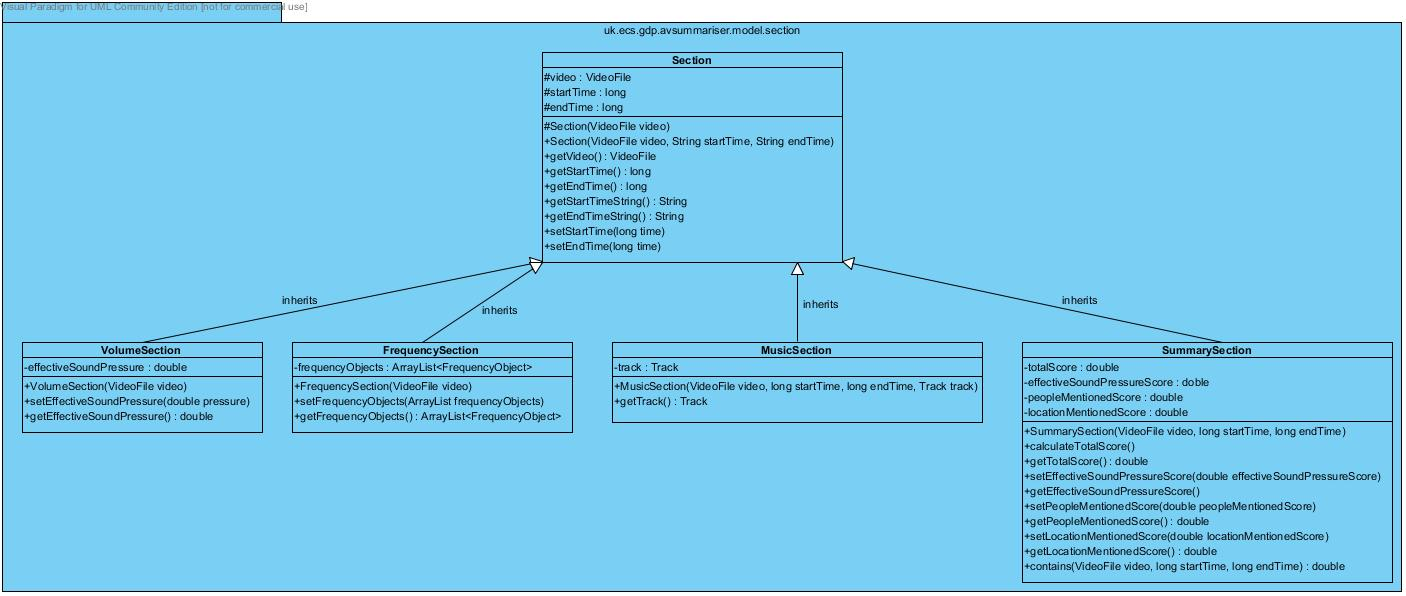
\includegraphics[trim = 0mm 0mm 0mm 0mm, clip,
 scale=0.28]{Images/section_package.jpg}
  \caption{The Section Package Diagram}\label{fig:sectionDiagram}
 \end{center}
\end{figure}

A Section object (the parent class) contains a VideoFile object and two longs values which are start and end times in milliseconds. These 
objects are used to define when something occurred in a video and the data that belongs to it, the additional information that the different 
objects contain are:

\begin{itemize}
	\item{VolumeSection - a double value for effective sound pressure (ESP) of this section.}
	\item{FrequencySection - an ArrayList of FrequencyObjects.}
	\item{MusicSection -  a Track object.}
	\item{SummarySection - four double values which represent ESP score, People mentioned score, Locations mentioned score and a total score.}
\end{itemize}

\newpage
\subsection{Software Libraries Used}

Before describing each of the modules, the software libraries that have been
used within this system and for what purposes they were used for are presented
in the table below.

\begin{tabular}{|p{135pt} | p{35pt} | p{230pt} | }
\hline
Software library / Resource name & Source & Usage \\\hline
OpenIMAJ & \cite{citeOpenImaj} & All modules \\\hline
JDOM & \cite{jdom} & XML parsing of subtitle files \& XML export of summary data \\\hline
OpenNLP  & \cite{nlp} & Natural language processing of subtitle files to find person's names and location's names \\\hline
Online TV Database & \cite{tvdb} & Open source database containing information about television programmes \\\hline
javatvdbapi & \cite{tvdbLibrary}  & API to communicate with thetvdb.com \\\hline
Echonest Music Intelligence Platform & \cite{citeEcho}  & Open system that provides a music identification service. \\\hline
jen-api & \cite{jenAPI} & API to communicate with Echonest platform. \\\hline
json-simple & \cite{jsonAPI} & Dependency for jen-api \\\hline
jfreechart & \cite{JFreeChart} & Produces graph of data for each video. \\\hline
\end{tabular}
\newpage 

\subsection{Online Television Database Integration}
\label{sec:TVDB}

\textbf{Package name: uk.ecs.gdp.avsummariser.model.tvdb.}

\subsubsection{Class Diagram}
The class diagram below details the structure of the classes within the package.

\begin{figure}[h1]
\begin{center}
 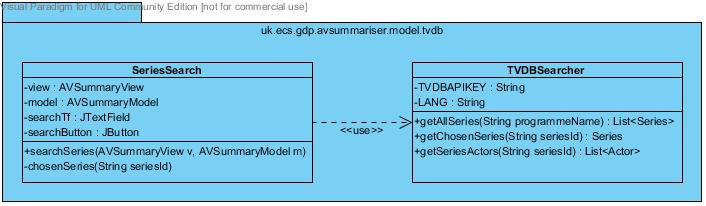
\includegraphics[trim = 0mm 0mm 0mm 0mm, clip,
 scale=0.5]{Images/tvdb_package_class_diagram.jpg}
  \caption{The tvdb Package Class Diagram}\label{fig:tvdbPackageClass}
 \end{center}
\end{figure}

The purpose of this package is to communicate with an open source database containing information about television programmes \ref{sec:TVDB} using the library javatvdbapi  \cite{tvdbLibrary}. The classes shown in figure \ref{fig:tvdbPackageClass} are explained further in the following sections:

\subsubsection{TVDBSearcher}
A static class used to communicate with the database and to gather all the necessary information such as:
\begin{itemize}
	\item{Obtain a list of Series (describes the television series such as its air date, a text overview and genres) objects given a search String.}
	\item{Obtain a Series object for the chosen television series.}
	\item{Obtain a list of Actor objects which represents the main characters for that series (each Actor object contains an actor name, character name and an image of the character).}	
\end{itemize}

\subsubsection{SeriesSearch}
A class called from the View and deals with the user's interaction, for example it presents a list of search results as a pop up message, sets the Model and updates the View after a user has chosen the television series. It uses the TVDBSearcher class to collect data from the database.

The information which this module gathers is used in Face Recognition (see Section \ref{sec:FacialRecognition}) and Name detection in subtitle files (see Section \ref{sec:PersonNameFinder}).

\newpage 
\subsubsection{User Walkthrough}
Below are two screenshots indicating how to link to the TV Database:

\textbf{Step 1:} Add video, type in the series name, press return and select available series. 
\begin{figure}[ht]
\begin{center}
 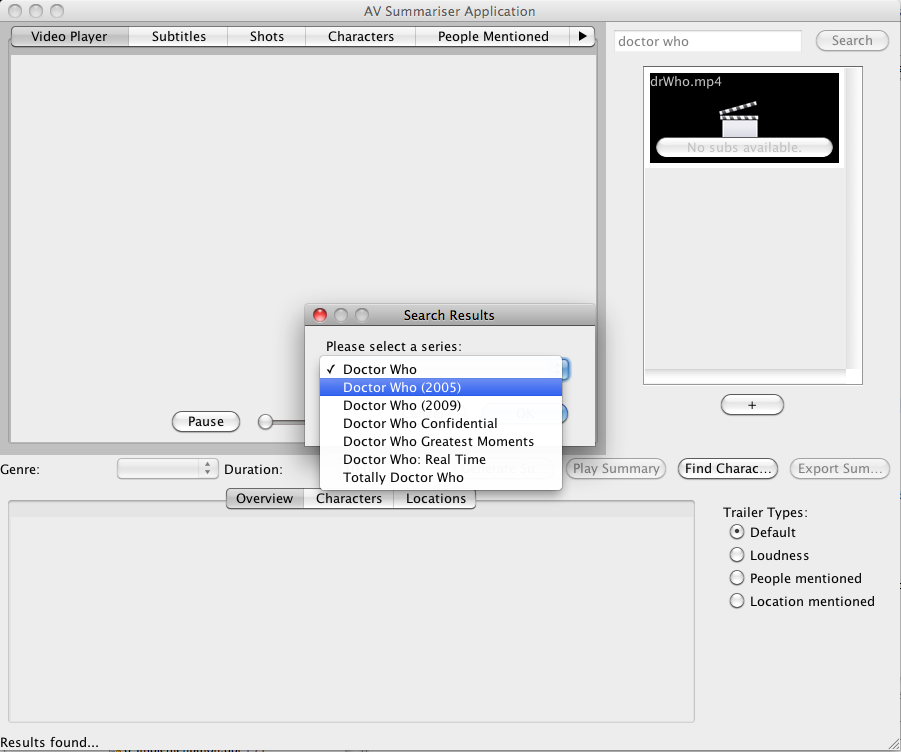
\includegraphics[scale=0.31]{Images/TVDBWalkthrough1.png}
  \caption{Selecting a Series}
 \end{center}
\end{figure}

\textbf{Step 2:} Press Generate Summary and the information is loaded into the Overview Tab. 
\begin{figure}[ht]
\begin{center}
 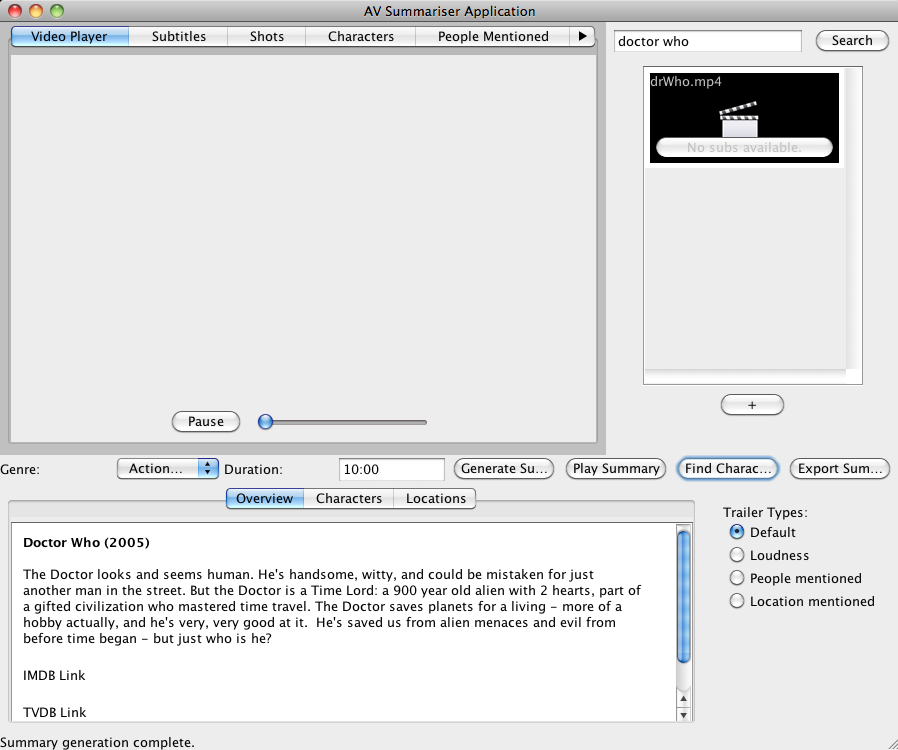
\includegraphics[scale=0.31]{Images/TVDBWalkthrough2.png}
  \caption{Viewing the Series Information}
 \end{center}
\end{figure}

\newpage

\subsection{Subtitles}
\label{sec:Subtitles}

\textbf{Package name: uk.ecs.gdp.avsummariser.model.subtitles}

The purpose of this package is to contain all of the Java code which interacts with the subtitle files that are associated with VideoFile objects. It performs:
\begin{itemize}
	\item{XML parsing of the subtitle files into the Subtitle Objects.}
	\item{Natural language processing to detect the main person's and location's names. This may include using data produced as a part of the Online Television Database Integration \ref{sec:TVDB}}
\end{itemize}

\subsubsection{Process Diagram}
A diagram of how these processes are chained together is given below:

\begin{figure}[h1]
\begin{center}
 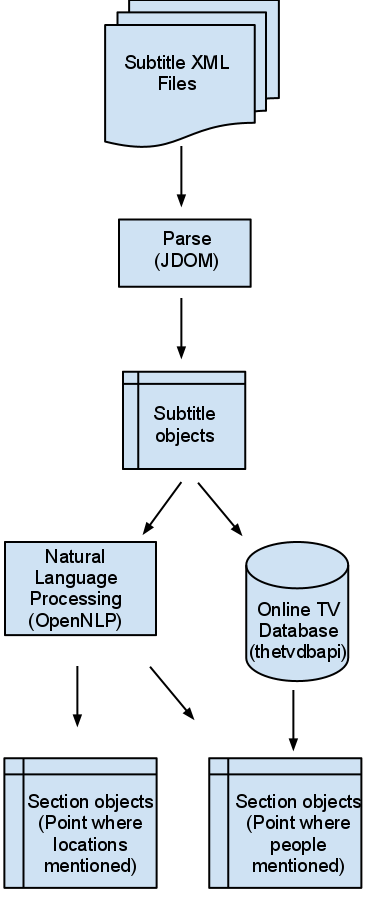
\includegraphics[trim = 0mm 0mm 0mm 0mm, clip,
 scale=0.45]{Images/Subtitleparsingprocess.png}
  \caption{The Subtitle Parsing Process Diagram}
 \end{center}
\end{figure}

\subsubsection{Class Diagram}
The structure of the classes used within this package are shown in the class diagram below with further detailed information following.

\begin{figure}[h1]
\begin{center}
 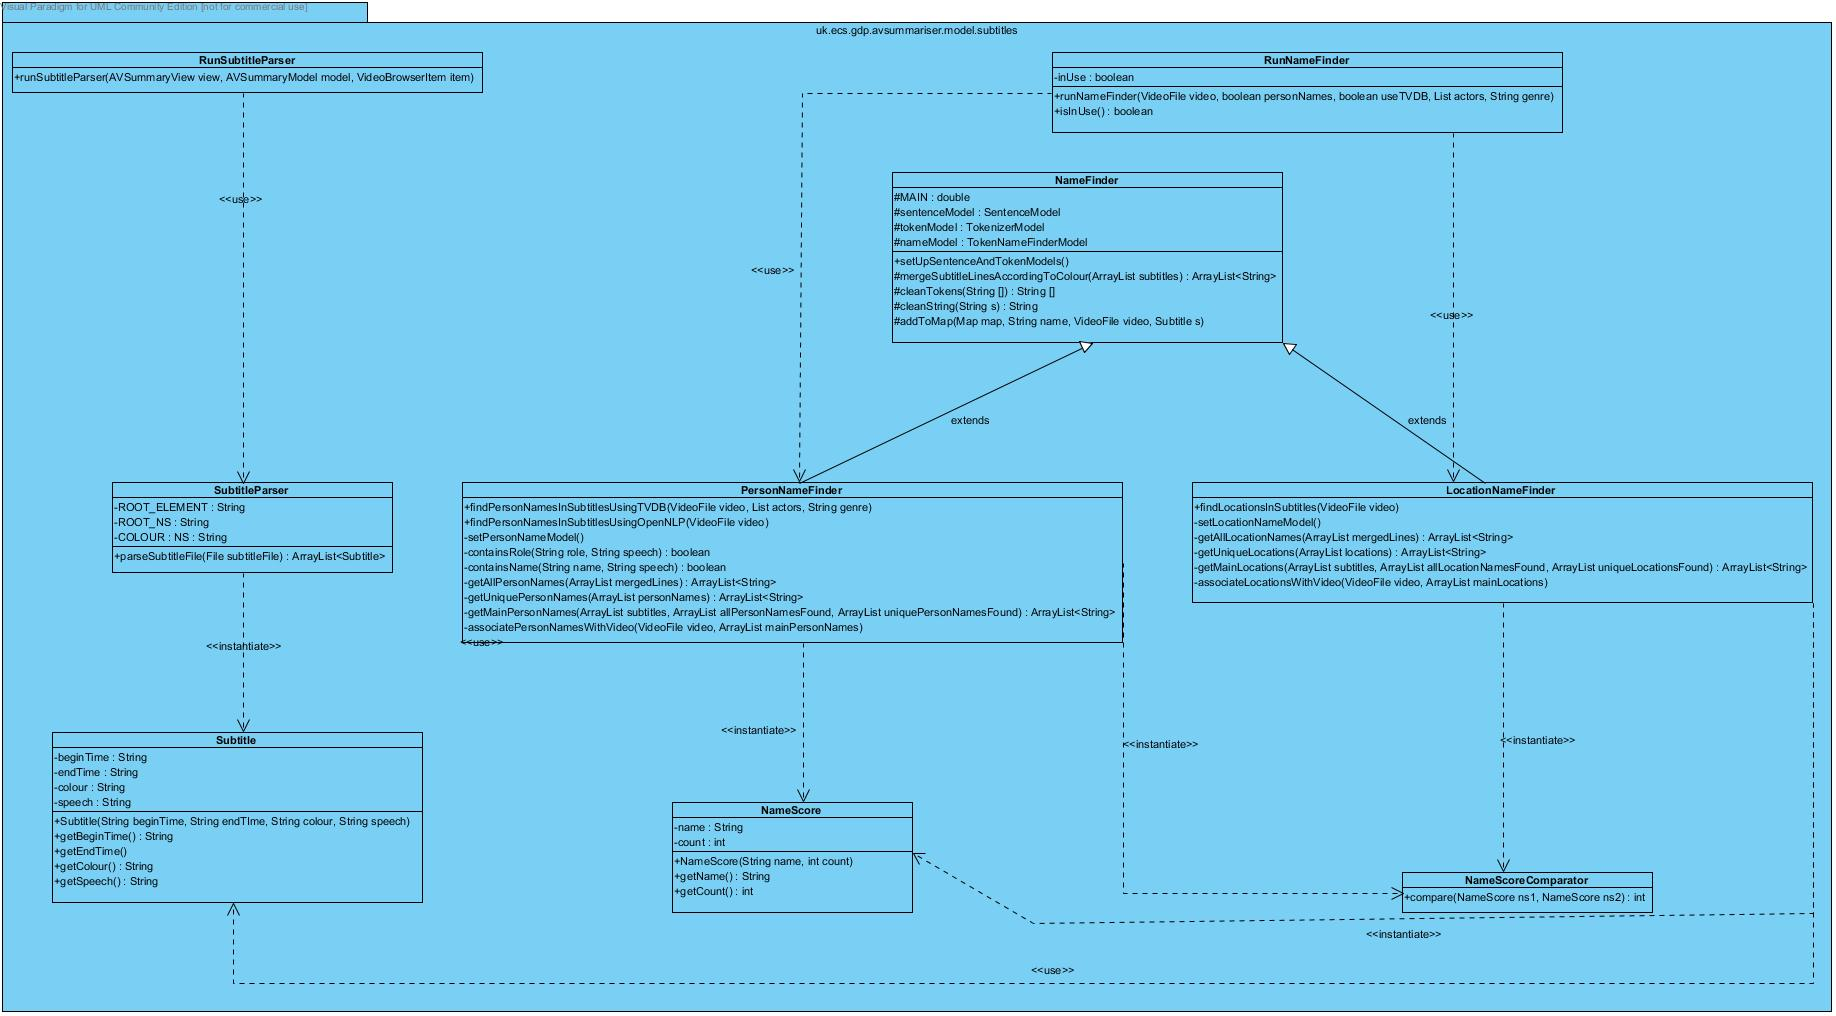
\includegraphics[trim = 0mm 0mm 0mm 0mm, clip,
 scale=0.24]{Images/subtitles_package_class_diagram.jpg}
  \caption{The Subtitles Package Class Diagram}\label{fig:subtitlesClassdiagram}
 \end{center}
\end{figure}

\newpage
\subsubsection{Subtitle}
This class represents an individual subtitle in a DVB subtitles file which contains a:
\begin{itemize}
	\item{Start time String.}
	\item{End time String.}
	\item{Speech String.}
	\item{Colour String which refers to a unique speaker in a video.}
\end{itemize}

\subsubsection{SubtitleParser}
This class parses an XML subtitle file (if it is of the correct format i.e. DVB format) to produce an ArrayList of Subtitle objects, which is done using the JDOM library \cite{jdom}.

\subsubsection{RunSubtitleParser}
This class is used to interact with the user when they select to load a subtitle file i.e. displaying a filechooser, updating the View and 
Model. This class then calls the SubtitleParser class to do the XML parsing.

\subsubsection{NameScore}
This class is used for name ranking purposes within the name finder classes below. It contains a String which is a name (e.g. person or 
location) that was found in the Subtitle Objects and a Integer which is a count of the number of times that name occurred in different 
Subtitle Objects.

\subsubsection{NameScoreComparator}
This is a class which implements the Comparator interface and is used to sort an ArrayList
of NameScore Objects in order of decreasing count value.

\subsubsection{NameFinder}
This class is the parent class for the PersonNameFinder and LocationNameFinder classes, it contains variables and methods that are common to both classes.

\subsubsection{PersonNameFinder}
\label{sec:PersonNameFinder}
A static class used to detect the main person names mentioned in an ArrayList of Subtitle
Objects. This can be done in either two ways; using natural language processing using the OpenNLP library \cite{nlp} or using information from the Online Television database Section \ref{sec:TVDB}: 

The natural language processing method works as follows:

\textbf{Stage 1:} Firstly, the speech variables in each Subtitle Object are merged together according to the String colour where they occur consecutively. This produces an ArrayList of String Objects.

\textbf{Stage 2:} Using the ArrayList produced previously, an ArrayList of String Objects containing all person names found is constructed by:
\begin{itemize}
	\item{Splitting each String Object into sentences.}
	\item{Splitting sentences into tokens.}
	\item{Tokens are then cleaned to remove punctuation and non speech items like ALARM SOUNDS.}
	\item{Finally, all person names are located.}
\end{itemize}

\textbf{Stage 3:} This ArrayList contains all person names so it is then analysed to produce an ArrayList containing all unique person names where full names take priority i.e. if this system detects a name, Ian, and another name, Ian Hislop, then in the unique names list it will only contain, Ian Hislop, and not, Ian.

\textbf{Stage 4:} For each unique name in this list the system counts how many times that name appears in the Subtitle Objects and creates a NameScore Object. These NameScore Objects are stored in another ArrayList. Next the ArrayList of NameScore Objects is sorted in descending order of count then the top 5\% of person names are chosen as the main people. 

\textbf{Stage 5:} Finally, using the main people's names and an ArrayList of Subtitle Objects, Section Objects are created for each occurrence of each main person name in the Subtitle Objects which is added to a Map object (where each String which is a main person name maps to a ArrayList of Section objects). Once this process has completed, the Map Object is associated with that video.

Alternatively to natural language processing, the system can use the information provided by the TVDB database which works as follows:

\textbf{Stage 1:} For each Subtitle Object it loops through the television series's Actor Objects and depending on the genre selected in the 
View either the character name or actor name Strings are used by the system and occurrences of these in each Subtitle Object are detected. 
Section Objects are created for each occurrence and adds it to a Map Object. Once this process has completed, the Map Object is associated 
with that video.

\subsubsection{LocationNameFinder}
A static class used to detect the main location names mentioned in an ArrayList of Subtitle Objects. Which is done using natural language processing using OpenNLP library \cite{nlp} and works as follows:

\textbf{Stage 1:} Firstly, the speech variables in each Subtitle Object are merged together according to the String colour where they occur consecutively. This produces an ArrayList of String objects.

\textbf{Stage 2:} Using the ArrayList produced previously, an ArrayList of String Objects containing all location names found is constructed by:
\begin{itemize}
	\item{Splitting each String Object into sentences.}
	\item{Splitting sentences into tokens.}
	\item{Tokens are then cleaned to remove punctuation and non speech items like ALARM SOUNDS. Finally, all location names are found.}
\end{itemize}

\textbf{Stage 3:} The ArrayList contains all the location names so it is then analysed to produce an ArrayList containing all unique location names.

\textbf{Stage 4:} For each unique location in the list the system counts how many times that location appears in the Subtitle objects and creates a 
NameScore Object. These NameScore Objects are stored in another ArrayList. Next the ArrayList of NameScore Objects is sorted in descending order of 
count, then the top 5\% of location names are chosen as the main locations. 

\textbf{Stage 5:} Finally, using the main location names and an ArrayList of Subtitle Objects the Section Objects are created for each occurrence of 
each main location name in the Subtitle Objects which is added to a Map Object (where each String which is a main location name maps to an ArrayList of Section Objects). 
Once this process has completed, the Map Object is associated with that video.

\subsubsection{RunNameFinder}
A class constructed to overcome the problems of the non thread safe TokenNameFinderModel and NameFinderME objects in OpenNLP \cite{nlp}, which throws a NullPointerException when different name finder threads are running i.e. one performing PersonNameFinder and another performing LocationNameFinder. Therefore this class was created to only allow one NameFinder process to run at a time.

\newpage 
\subsubsection{User Walkthrough}
Below are two screenshots indicating how to load in the subtitles:

\textbf{Step 1:} Add video, select the subtitles section and add the appropriate subtitles. 
\begin{figure}[ht]
\begin{center}
 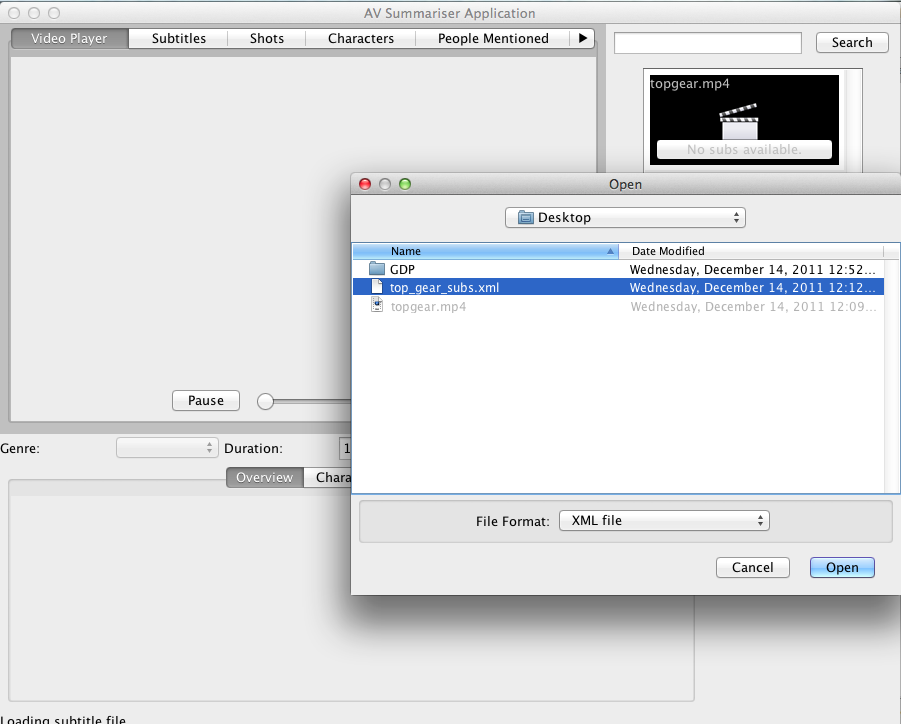
\includegraphics[scale=0.31]{Images/SubtitleWalkthrough1.png}
  \caption{Adding Subtitles to a Video}
 \end{center}
\end{figure}

\textbf{Step 2:} Select the video and the subtitles are loaded into the the Subtitles tab. 
\begin{figure}[ht]
\begin{center}
 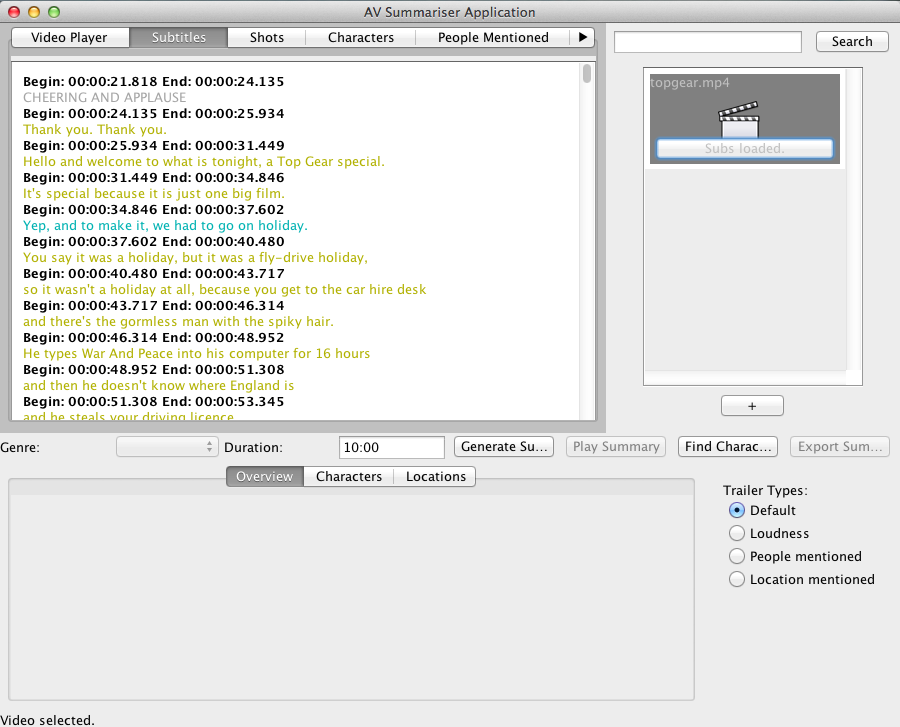
\includegraphics[scale=0.31]{Images/SubtitleWalkthrough2.png}
  \caption{Viewing the Subtitles}
 \end{center}
\end{figure}

\newpage

\newpage
\subsection{Audio Processing}
\label{sec:AudioProcessing}

\textbf{Packages:}
\begin{itemize}
	\item{\textbf{uk.ecs.gdp.avsummariser.model.audio}}
	\item{\textbf{uk.ecs.gdp.avsummariser.model.music}}
\end{itemize}

The purpose of this package is to contain all the Java code which processes the audio of video files. This has been implemented using the OpenIMAJ 
library \cite{citeOpenImaj} and for an audio stream it:
\begin{itemize}
	\item{Determines the loud sections and produces an ArrayList of VolumeSection Objects.}
	\item{Determine the frequency and intensity of an audio stream and produces a list of FrequencySection Objects.}
	\item{Identify music sections.}
\end{itemize}

\subsubsection{Process Diagram}
A diagram of how this process chains together is given below:

\begin{figure}[h1]
\begin{center}
 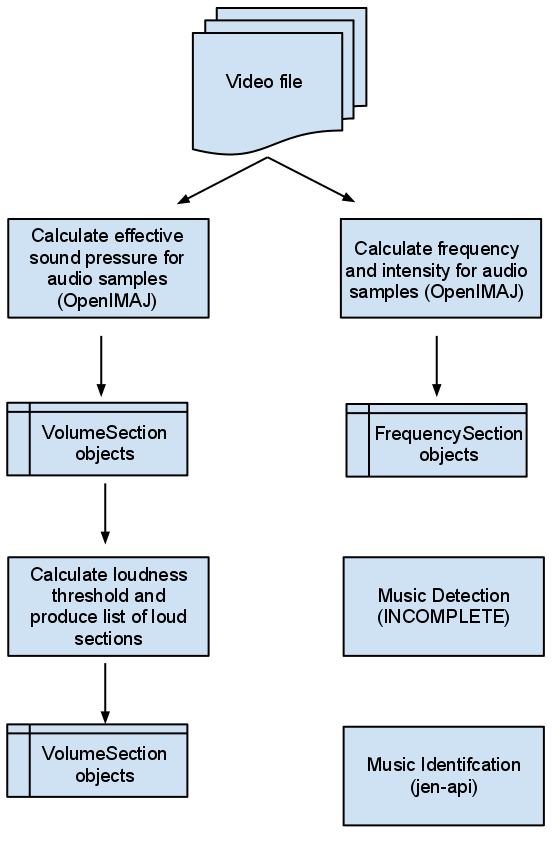
\includegraphics[trim = 0mm 0mm 0mm 0mm, clip,
 scale=0.4]{Images/Audioparsingprocess.png}
  \caption{The Audio Parsing Process Diagram}
 \end{center}
\end{figure}

\newpage

\subsubsection{Class Diagram}
The structure of the classes used within this package are shown in the following class diagrm:

\begin{figure}[h1]
\begin{center}
 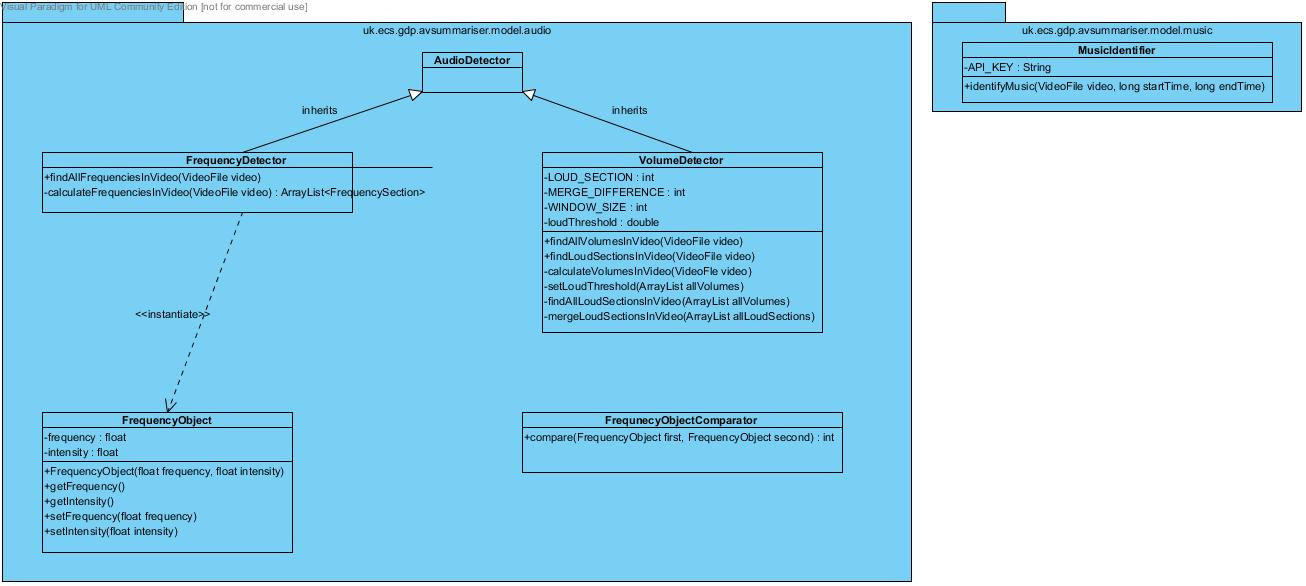
\includegraphics[trim = 0mm 0mm 0mm 0mm, clip,
 scale=0.33]{Images/audio_package_class_diagram.jpg}
  \caption{The Audio Processing Package Class Diagram}
 \end{center}
\end{figure}

\subsubsection{FrequencyObject}
A class used to store the frequency and intensity float values for each Fast Fourier Transform value calculated from an audio sample. An ArrayList of these Objects are stored within each FrequencySection Object.

\subsubsection{FrequencyObjectComparator}
A class which implements the Comparator interface and is used to sort an ArrayList
of FrequencyObject Objects in an ascending order of frequency value.

\subsubsection{VolumeDetector}

A static class used to calculate the effect sound pressure (ESP) of the audiosample and determine the loud sections, this is done in the following way:

\textbf{Stage 1:} For an audio stream, the system samples it into chunks and calculates the ESP for that chunk and creates a VolumeSection Object. This produces an ArrayList of VolumeSection Objects for the entire video.

\textbf{Stage 2:} Next using this ArrayList, it sorts the VolumeSection Objects in descending order of the ESP values and then selects the index of the last VolumeSection Object in the top 1\%, the value of this Object will be the loud threshold.

\textbf{Stage 3:} Now the VolumeSection Objects are looped through in time order and any Object with ESP value greater than or equal to the loud threshold is kept, so now there is a ArrayList of loud sections.

\textbf{Stage 4:} Finally, these loud VolumeSection Objects are then merged if they are within a second of one another to produce the finalised ArrayList of VolumeSection Objects, which are then associated with a video. 

\subsubsection{FrequencyDetector}
A static class used to calculate the frequency of audio samples within an audio stream of a video file. The calculation of the frequency of audio samples is done in the following way:

\textbf{Stage 1:} For an audio stream, the system samples it as chunks and performs the Fast Fourier Transform (FFT) for each chunk. For each value produced by the FFT it works out its frequency and intensity and creates a FrequencyObject Object. Then a FrequencySection is created for that chunk and it contains an ArrayList of FrequencyObject Objects. Once this process is completed, an ArrayList of FrequencySection Objects is associated with that video.

The second purpose of the class was to then use the data calculated above to detect if and where music occurred in an audio stream of a video. However this section of the detector is incomplete for a 
number of reasons firstly is that the team was unable to find any suitable libraries to perform this process. The set of tools called 
jMIR \cite{JMIR} which was found to include JAudio \cite{JAudio}, however the documentation was hard to understand and no tutorials were found therefore it 
was hard to judge whether it was fit for purpose and so no use to the system. Therefore, as per the risk strategy defined in Section \ref{sec:Risks}, the team opted to try 
and implement our own solution. Firstly a process of detecting frequency patterns was constructed to detect music although this became apparent 
that it wasn’t generalized and only worked for the example that it was being tested on. The next attempt was using beat detection, prior to 
OpenIMAJ’s addition of BeatDetector, the Frequency selected sound energy algorithm detailed in this paper \cite{BeatDetection} was chosen to be 
implemented due to FFT being implemented in OpenIMAJ already. However after testing this method it was also unsuccessful. 

Due to the time restrictions of the project and the lack of successful results, this part of the class is incomplete and therefore has formed part of 
our future work, shown in Section \ref{sec:FutureWork}. Furthermore, the frequency detection has not been integrated into the final product although the code exists within the system.

\subsubsection{Music Identifier}
\label{sec:Music}
A static class used to communicate with the EchoNest service \cite{citeEcho} to identify music using the jen-api \cite{jenAPI}. This works in the following way:

\textbf{Stage 1:} Given a VideoFile Object and a start and end time in milliseconds, it creates a new temporary video file for that specified segment.

\textbf{Stage 2:} This file is then uploaded to the EchoNest service for analysis then one of the following can occur:
\begin{itemize}
	\item{If the analysis completes and is successful in identifying, the track object which contains information such as the artist's name, song's title and the album's name is returned.}
	\item{If the analysis completed and is unsuccessful in identifying so a Track object is returned, but with all information set to null.}
	\item{Finally, if the analysis fails then nothing is returned.}
\end{itemize}
\textbf{Stage 3:} Then using either a Track Object or null, a MusicSection Object is created containing the video used, the times specified as well as the Track or null Object.

\newpage
\subsection{Facial Recognition}
\label{sec:FacialRecognition}

\textbf{Package: uk.ecs.gdpavsummariser.model.facialdetection}

\subsubsection{Face Detection Techniques}
Before describing the different classes in this section, the systematic set of techniques used to produce these final classes and the findings made throughout the duration of the project are detailed.

\textbf{Simple Face Detection}
\newline
Initially the face recognition section purely dealt with identifying faces, it used a face detector from the OpenIMAJ library \cite{citeOpenImaj} to run through the frames of the video and pick out and draw the faces that were found.

\begin{figure}[h1]
\begin{center}
 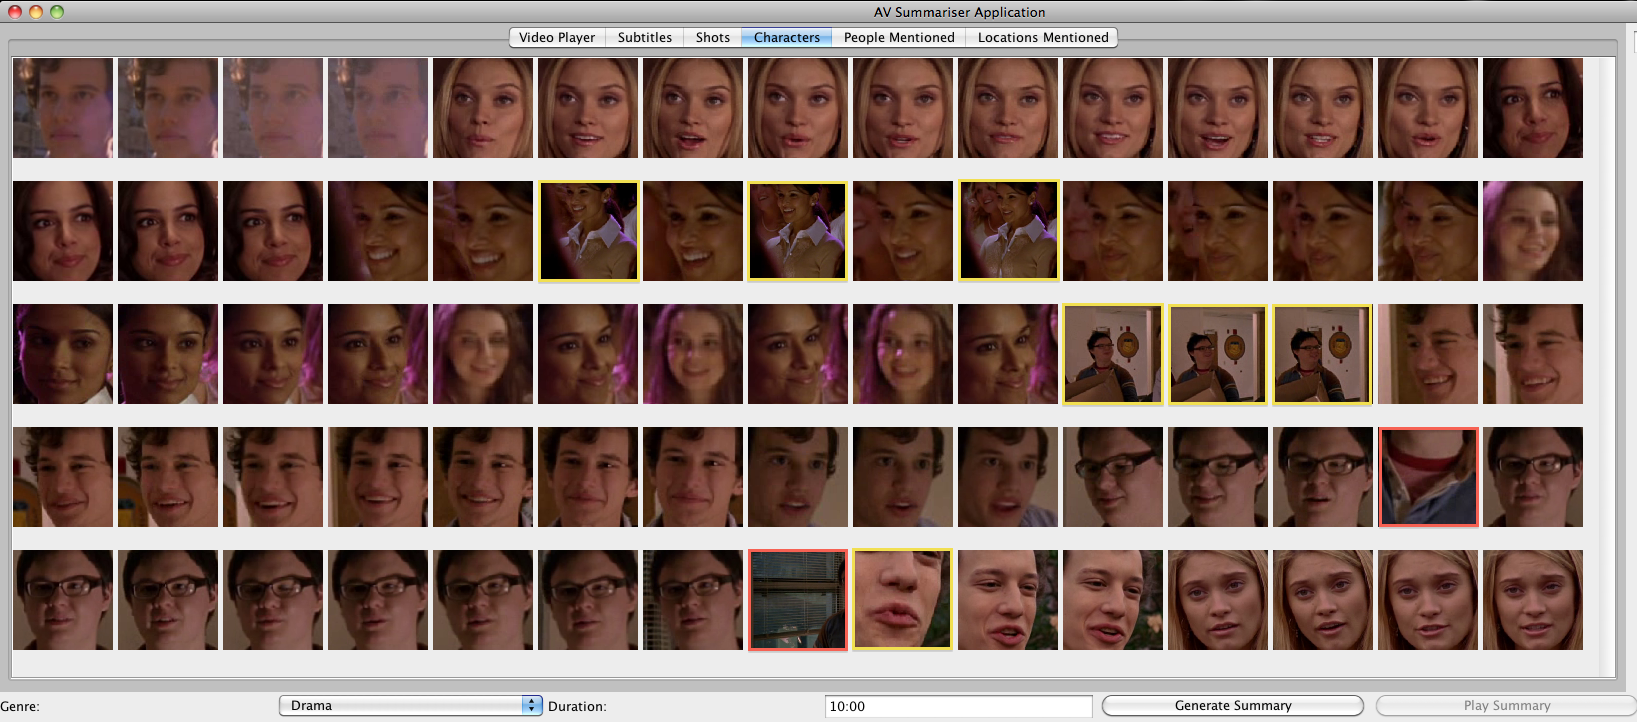
\includegraphics[trim = 0mm 0mm 0mm 0mm, clip,
 scale=0.265]{Images/GreekFacialDetection.png}
  \caption{Greek Facial Detection}
 \label{fig:GreekFD}
 \end{center}
\end{figure}

\begin{figure}[h1]
\begin{center}
 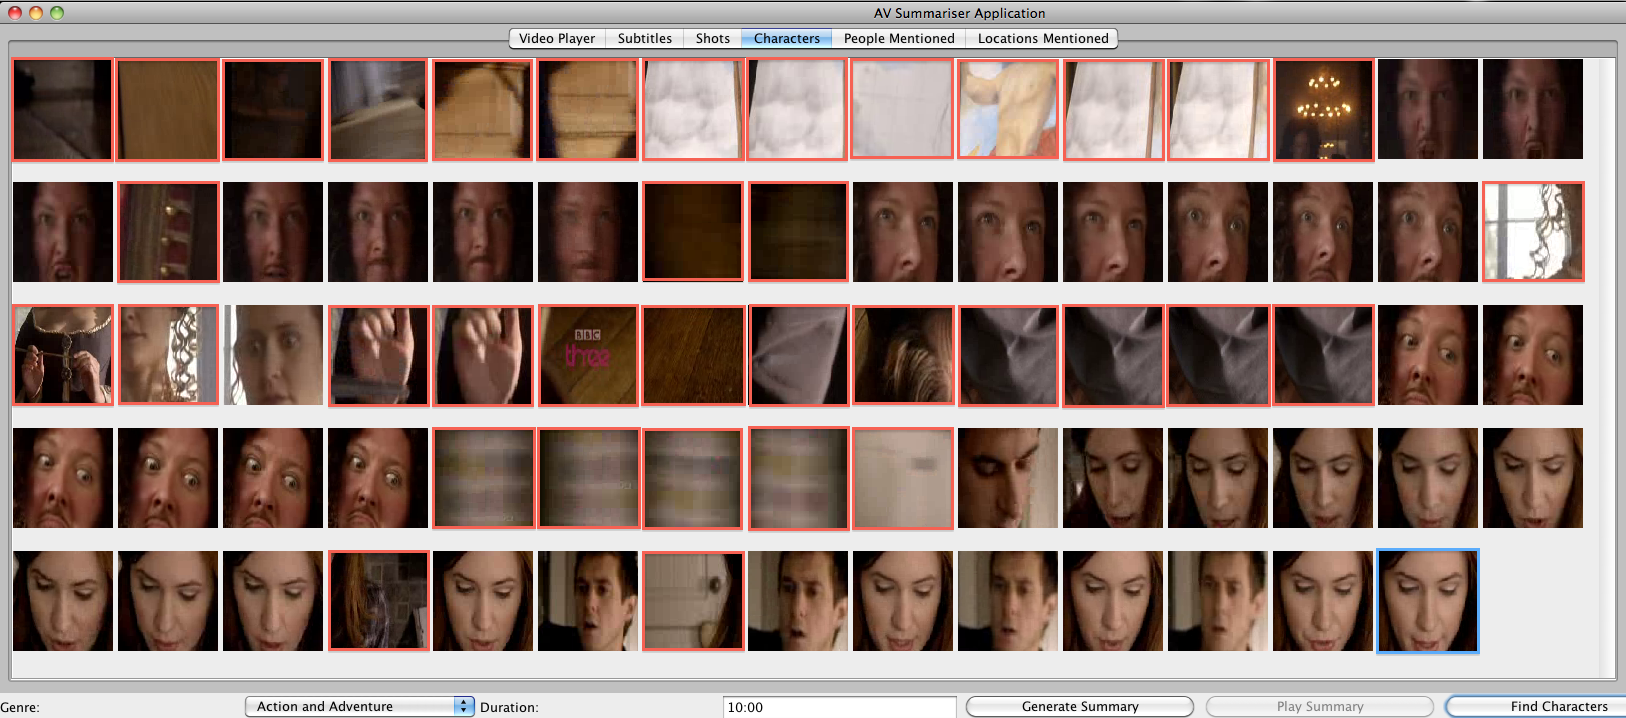
\includegraphics[trim = 0mm 0mm 0mm 0mm, clip,
 scale=0.265]{Images/DrWhoFacialDetection.png}
  \caption{Doctor Who Facial Detection}
 \label{fig:DrWhoFD}
 \end{center}
\end{figure}

\newpage

As you can see from the images above in each instance there are still some false positives coming through (although significantly less in Figure \ref{fig:GreekFD}). Following are the statistics of the percentage of correctly extracted faces from the previous images.

\begin{figure}[h1]
\begin{minipage}[b]{0.5\linewidth}
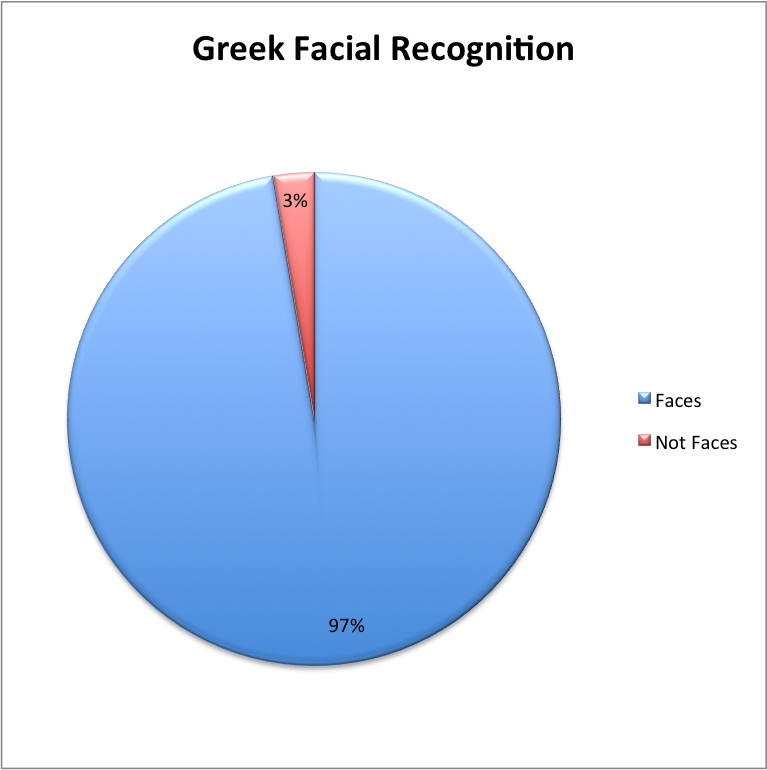
\includegraphics[scale=0.55]{Images/GreekFaces1.png}
\caption{Greek Pie Chart}
 \label{fig:GreekFD}
\end{minipage}
\hspace{0.5cm}
\begin{minipage}[b]{0.5\linewidth}
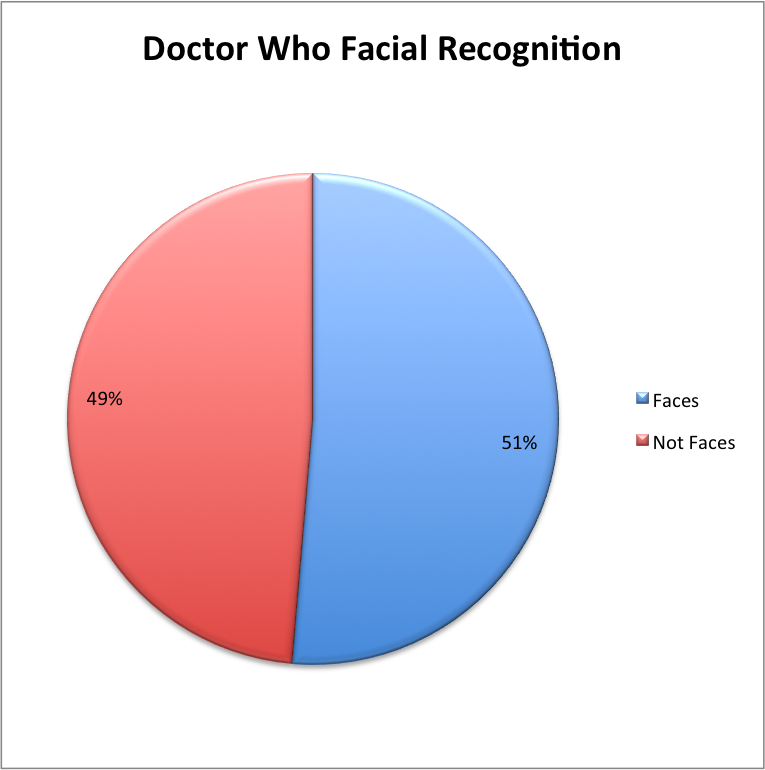
\includegraphics[scale=0.55]{Images/DrWhoFaces1.png}
\caption{Doctor Who Pie Chart}
 \label{fig:DrWhoFD}
\end{minipage}
\end{figure}

As can be seen from the pictures above, this produced varied results based on the genre of the video. A light comedy video as displayed in Figure \ref{fig:GreekFD} produced significantly better results than a poorly lit, action filled video as displayed in Figure \ref{fig:DrWhoFD}. 

\textbf{Advanced Face Detection}
\newline
In order to achieve advanced face detection a minute of footage was gone through looking at every fifth frame and each detected face that was collected within these frames was logged as either a specific character match or a non-character. It is well known that facial detection is not an exact science and that when faces aren't fully frontal facing in good lighting conditions its extremely difficult to identify them accurately. Therefore its unsurprising that whilst the OpenIMAJ library detects a majority of the faces that appear in the video occasionally other objects get detected as faces also. Therefore these methods were ran to attempt to determine the following: 

\begin{itemize}
	\item{How to tell if a detected face was actually a face.}
	\item{How to tell if two faces were actually the same person.}
\end{itemize} 

OpenIMAJ provides methods to create histograms of images and to compare these for similarity. These methods can be ran with various different 
parameters such as different types of detected faces, and different aligners to try and match the images. To gather statistics these methods were 
ran with the aligner that were deemed most appropriate and some interesting results were produced. Whilst looking at the different values produced 
for the different characters it didn't give any real indication of scale, looking at the correlation between faces and false positives gave some more 
useable results:

\begin{center}
\begin{table}[ht]
\begin{tabular}{|p{131pt}|p{131pt}|p{131pt}|}
	\hline
	& Min Value & Max Value \\\hline
	True Faces & 7.23 & 11.62 \\\hline
	False Faces & 7.61 & 17.29 \\\hline
\end{tabular}
\caption{Correlations between faces and false positives}
\end{table}
\label{tab:faceFalsePositive} 
\end{center}

These results show that all the actual faces only come within a certain range of values, despite the false positives also producing values within that range, they also produced
values that are significantly outside it. Using these results, any detected face that came outside the boundary that was likely to be a face was discarded. The 
face detection was then ran with various boundary values based off these statistics. Below are some pictures illustrating that. In each picture the 
incorrectly identified faces are outlined in red, and a common face to all images is outlined in blue to show the difference in facial extraction per 
the same number of frames. 

\begin{figure}[h1]
\begin{center}
 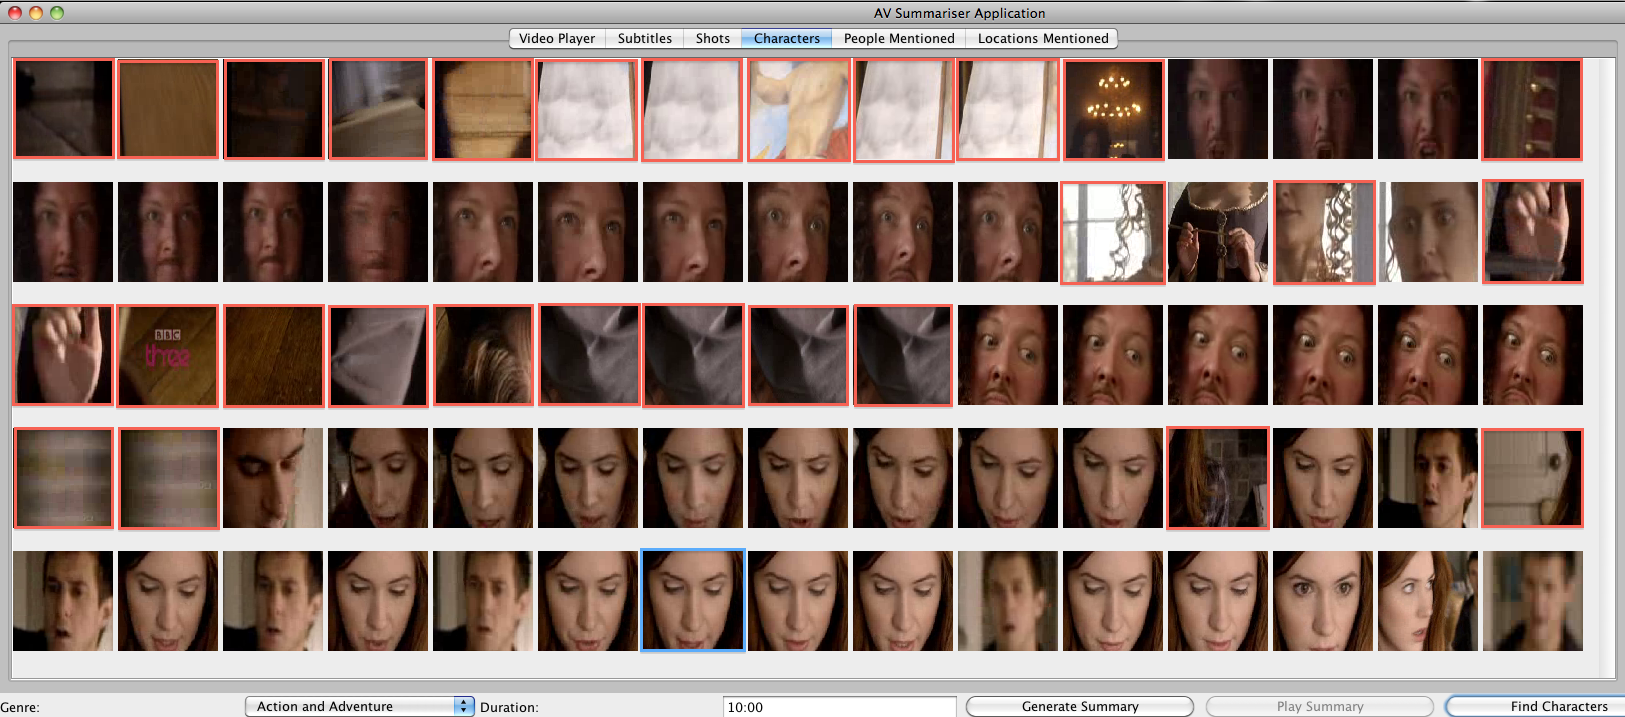
\includegraphics[trim = 0mm 0mm 0mm 0mm, clip,
 scale=0.19]{Images/sevenpointfivetoelevenpointfive.png}
  \caption{Facial Detection on Doctor Who: min value = 7.5 \& max value = 11.5}
 \end{center}
\end{figure}

\begin{figure}[h1]
\begin{center}
 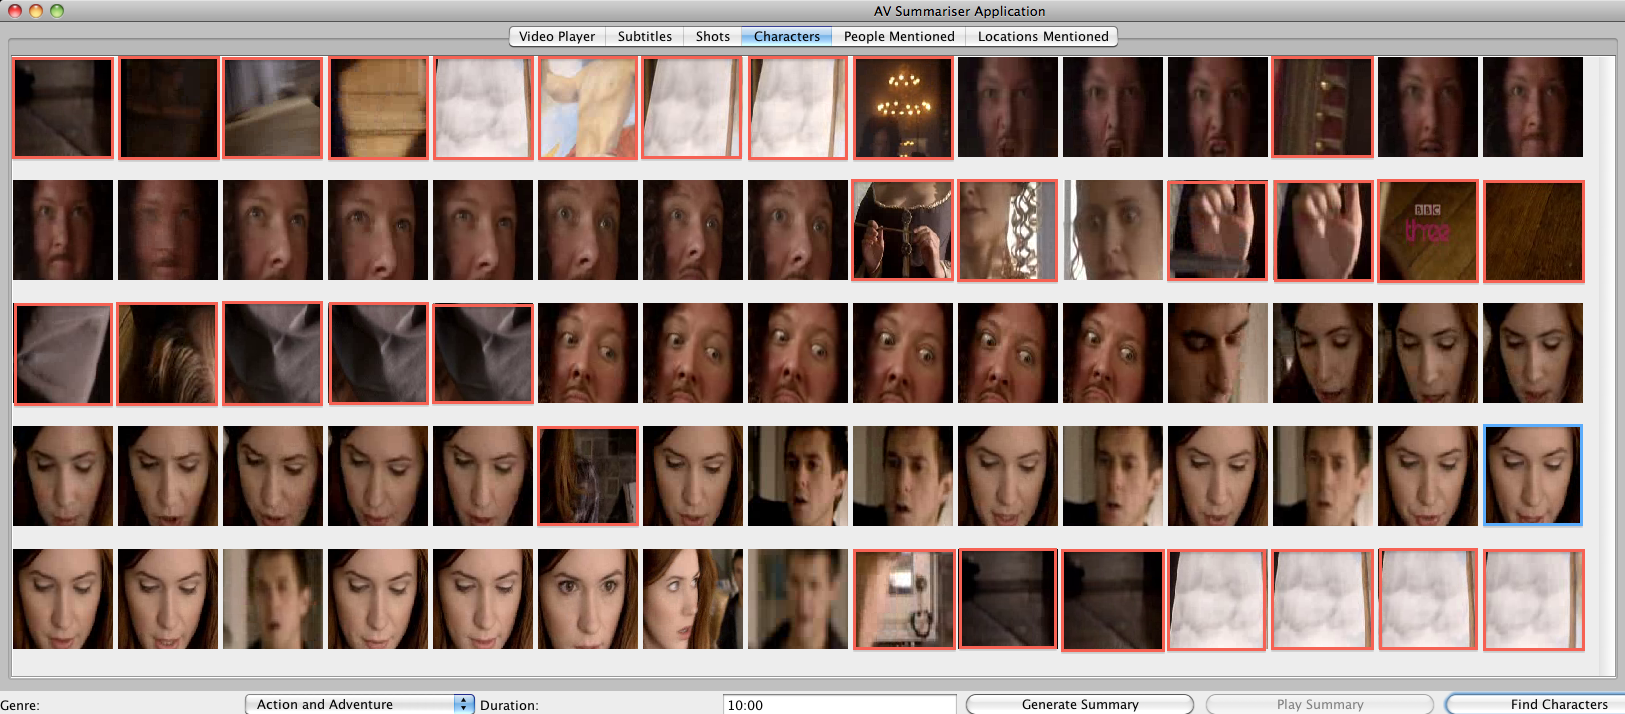
\includegraphics[trim = 0mm 0mm 0mm 0mm, clip,
 scale=0.19]{Images/seveneightninetoeleven.png}
  \caption{Facial Detection on Doctor Who: min value = 7 or 8 or 9 \& max value = 11}
 \end{center}
\end{figure}

\begin{figure}[h1]
\begin{center}
 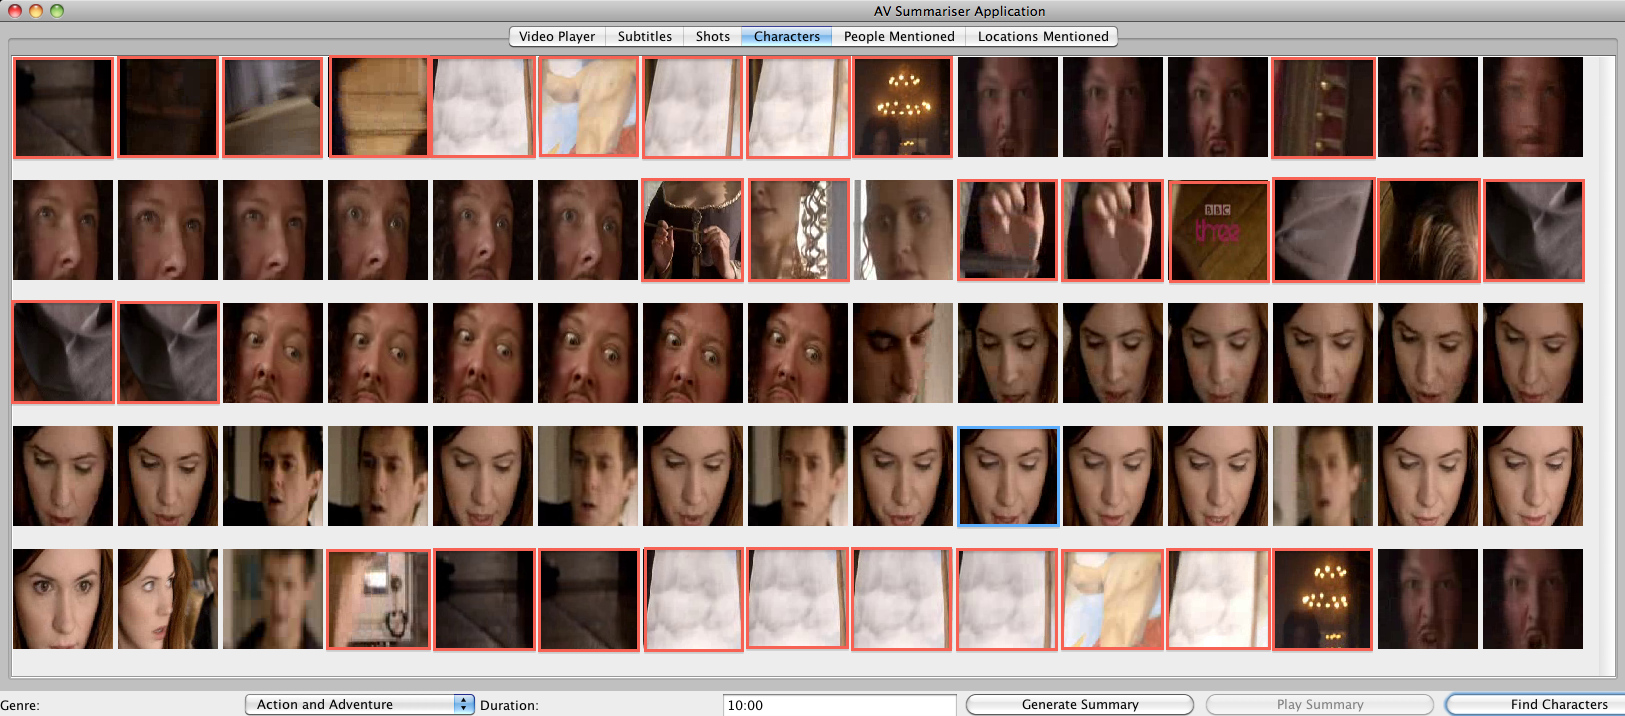
\includegraphics[trim = 0mm 0mm 0mm 0mm, clip,
 scale=0.19]{Images/tentoeleven.png}
  \caption{Facial Detection on Doctor Who: min value = 10 \& max value = 11}
 \end{center}
\end{figure}

\newpage

\begin{figure}[h1]
\begin{center}
 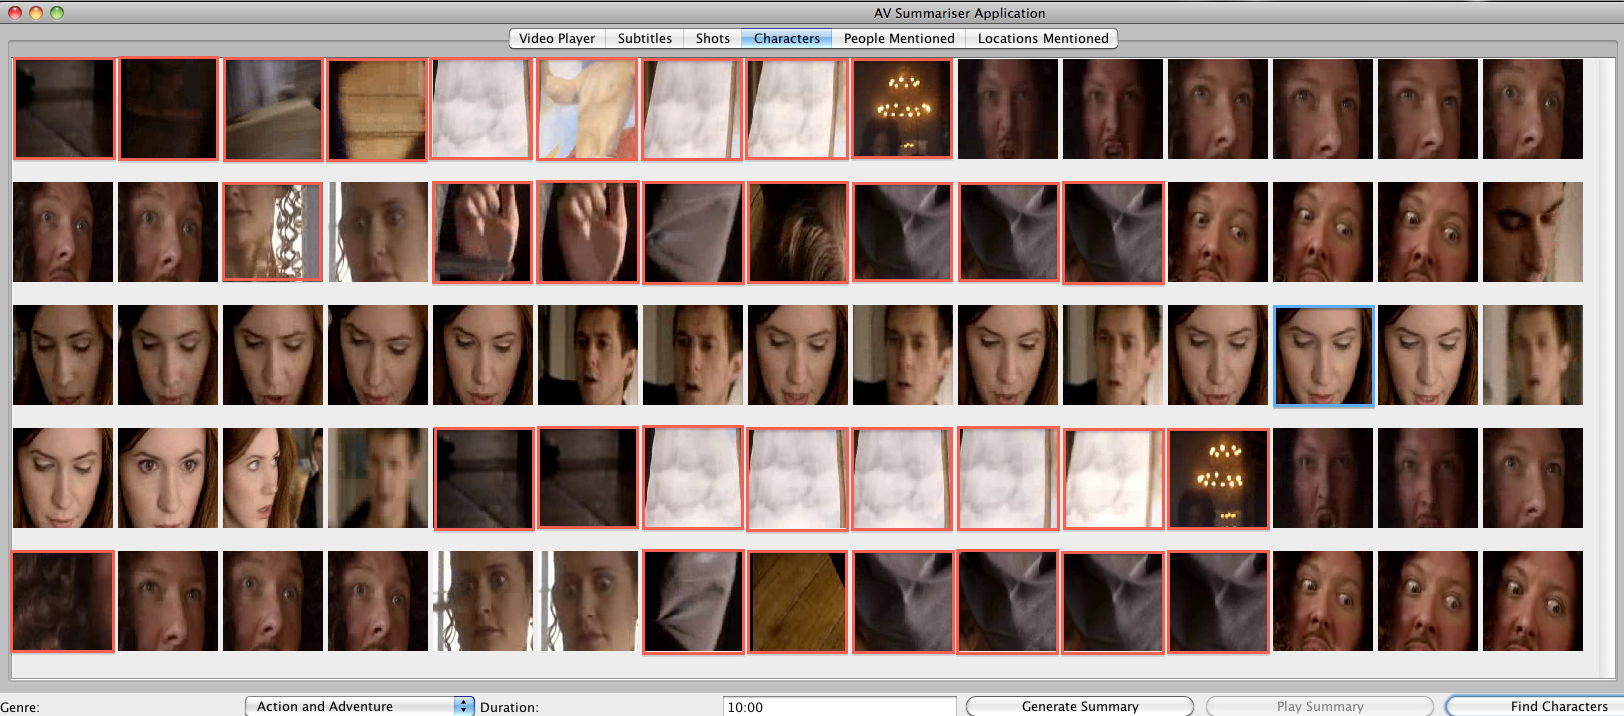
\includegraphics[trim = 0mm 0mm 0mm 0mm, clip,
 scale=0.19]{Images/tenpointtotoeleven.png}
  \caption{Facial Detection on Doctor Who: min value = 10.2 \& max value = 11}
 \end{center}
\end{figure}

These pictures show that by adjusting these ranges different images will be registered as faces. However, it is difficult to tell from these images which method is the most accurate in terms of getting the highest percentage of positive faces. It is also misleading to solely judge this by the percentage of matches displayed in the panel as two ranges could produce the same numbers but different sets of images. Below is a table that shows the ranges against the percentage of faces in the panel as a whole and the percentage of faces in a set of frames common to all experiments. 

\begin{table}[ht]
\begin{tabular}{|p{50pt} | p{80pt} | p{80pt} | p{80pt} | p{80pt} | }
\hline
Histogram Range & No Faces that fill the panel & \% Faces that fill the panel & No Faces in common frames & \% Faces in common frames \\\hline
None	&38/74	&51.3\%	&38/74	&51.3\% \\\hline
7.5-11.5	&46/75	&61.3\%	&38/67	&56.7\% \\\hline
7-11	&46/75	&61.3\%	&38/60	&63.3\% \\\hline
8-11	&46/75	&61.3\%	&38/60	&63.3\% \\\hline
9-11	&46/75	&61.3\%	&38/60	&63.3\% \\\hline
10-11	&45/75	&60.0\%	&35/55	&63.6\% \\\hline
10.2-11	&43/75	&57.3\%	&26/43	&60.5\% \\\hline
\end{tabular}
\caption{Ranges and Percentages of Faces}
\end{table}
\label{tab:RangesAndPercentages} 

These results show that looking purely at the percentage of faces that fill the panel it would be most efficient in terms of getting the highest 
percentage of matches to use the range 7.5-11.5 or 7/8/9-11. However, the percentage of matches in the common frames suggests that the most 
accurate range to use is 10-11, supported by the fact that it had the same number of face matches as the wider ranges of 7/8/9-11, but it had 8 less false positives. Therefore that range is the one that is used in the final face detection methods.

An additional technique that was added to this for the darker programmes was a pixel comparison method. The middle square of each face was compared to get its mean value and statistics were run in the same way as above and the results were as follows: 

\begin{center}
\begin{table}[ht]
\begin{tabular}{|p{70pt} | p{75pt} | p{75pt} | p{75pt} | p{75pt} | }
	\hline
	& X Min Value & X Max Value & Y Min Value & Y Max Value \\\hline
	True Faces & 0.000000059 & 0.89 & 0.000000029 & 0.85 \\\hline
	False Faces & 0.0 & 0.98 & 0.0 & 0.98 \\\hline
\end{tabular}
\caption{X and Y Values of True and False Faces}
\end{table}
\label{tab:TrueFalseValues} 
\end{center}

\newpage
Following the same pattern as above two different range of x,y values were tried and below are the pictures to illustrate this experiment.

\begin{figure}[h1]
\begin{center}
 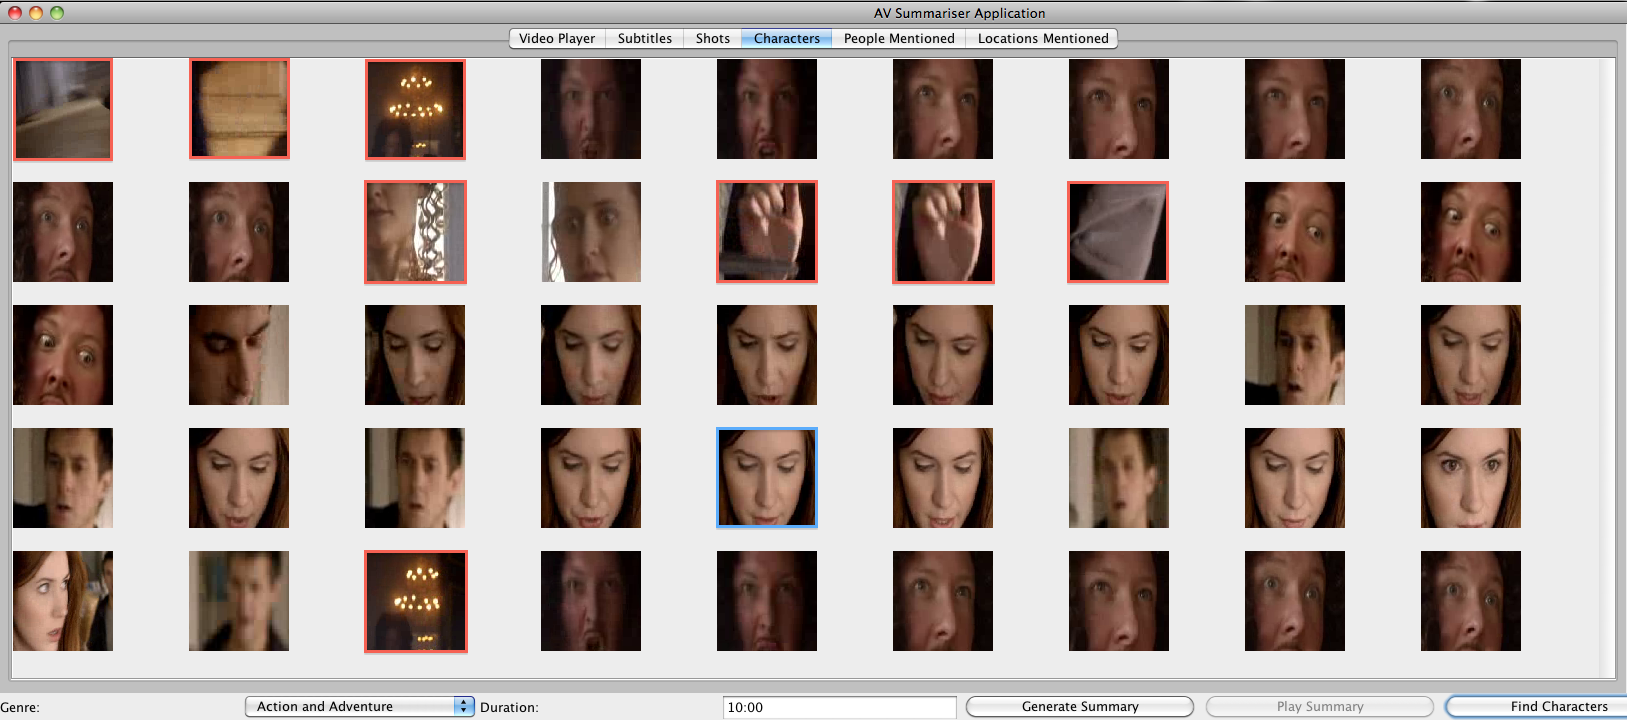
\includegraphics[trim = 0mm 0mm 0mm 0mm, clip,
 scale=0.19]{Images/pixels0208.png}
  \caption{Facial Detection on Doctor Who: min x,y value = 0.2 \& max x,y value = 0.8}
 \end{center}
\end{figure}

\begin{figure}[h1]
\begin{center}
 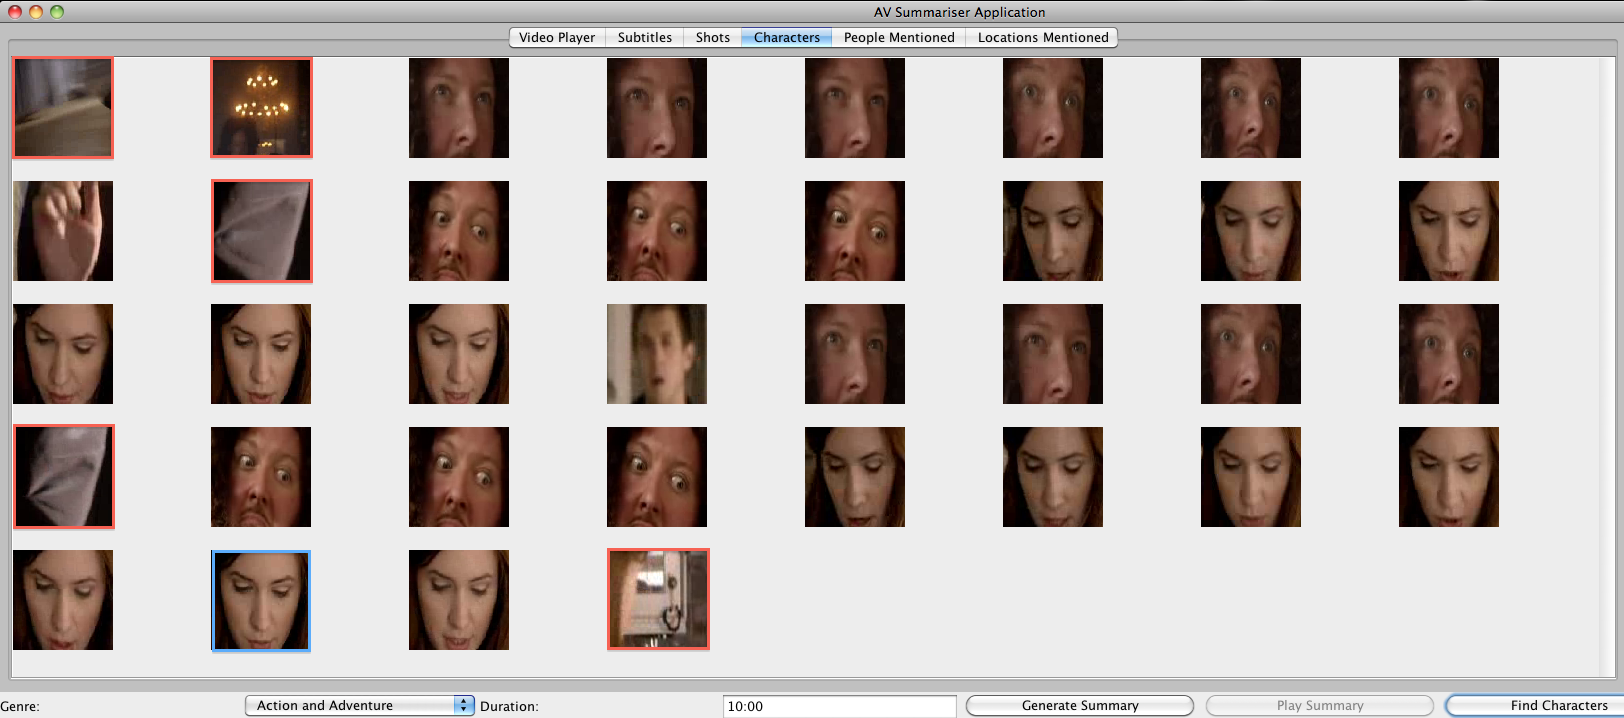
\includegraphics[trim = 0mm 0mm 0mm 0mm, clip,
 scale=0.19]{Images/pixels0306.png}
  \caption{Facial Detection on Doctor Who: min x,y value = 0.3 \& max x,y value = 0.6}
 \end{center}
\end{figure}

As you can see from the pictures above these are primarily now made up of faces with a lot of the false positives irradicated. However, whilst this stricter method makes for a set of almost all faces, it still throws away some positive matches. Below is a table of stats to reflect these images. 

\begin{table}[ht]
\begin{tabular}{|p{40pt} | p{82pt} | p{83pt} | p{82pt} | p{83pt} | }
\hline
X,Y Values & No Faces that fill the panel & \% Faces that fill the panel & No Faces in common frames & \% Faces in common frames \\\hline
0.3,0.6	&29/36	&80.5\%	&28/37	&75.6\% \\\hline
0.2,0.8	&37/45	&80.0\%	&25/32	&78.1\% \\\hline
\end{tabular}
\caption{Face Data for previous Figures}
\end{table}
\label{tab:PreviousFigures} 

As you can see above, when comparing the common set of frames the wider range proves more accurate and still keeps a majority of the 
faces detected in the methods described above. It is debatable as to whether it is a worthwhile trade to throw away some positive matches in 
exchance for reducing the amount of false positives. The reasoning here has been that because facial clustering is such a hard problem, to 
maximise the chances of accuracy it would help to work from a set of accurately judged faces. In addition to this the data this section aims 
to produce for the summary is a log of a character's appearances and a set of timestamps where it is very likely that a character is in that frame. 
Therefore this method was implemented as an additional step for the darker programmes under the genres of ``Action \& Adventure" and ``Science-fiction".

\newpage
\textbf{Face Clustering}
\newline
After refining the facial detection techniques, the next stage was to attempt to cluster them. Four different techniques were tried to cluster the faces successfully:
\begin{itemize}
	\item{SIFT Comparison of Facial Keypoints}
	\item{Histogram Comparison using an aligner to account for faces in different positions}
	\item{Pixel Comparison of the center and boundary areas of the detected faces}
	\item{SIFT Comparison of Image Keypoints}
\end{itemize}

All of these techniques were tried on the lighter comedy video to see how well the clustering would work on an easier video first before looking into darker videos. 

\textbf{SIFT Comparison of Facial Keypoints:} Using this method the different facial keypoints (e.g mouth and nose) were compared using a SIFT 
Comparator, similar to the method described in L. Ballan et al. paper \cite{football}. On paper this seemed like the obvious solution but in practice it was 
very difficult to construct a scale from the returned values to ascertain what made a match. Therefore this technique was quickly abandoned.

\textbf{Histogram Comparison using an aligner to account for faces in different positions:} This technique uses the same principles as the one mentioned above in regards to advanced face detection. However, instead of working on a range, this technique tried to pinpoint how close the image match results were to the middle of the given scale, reasoning that this might be the way to identify matches within the different faces. A screenshot showing the data gathered from this attempt is shown below:

\begin{figure}[ht]
\begin{center}
 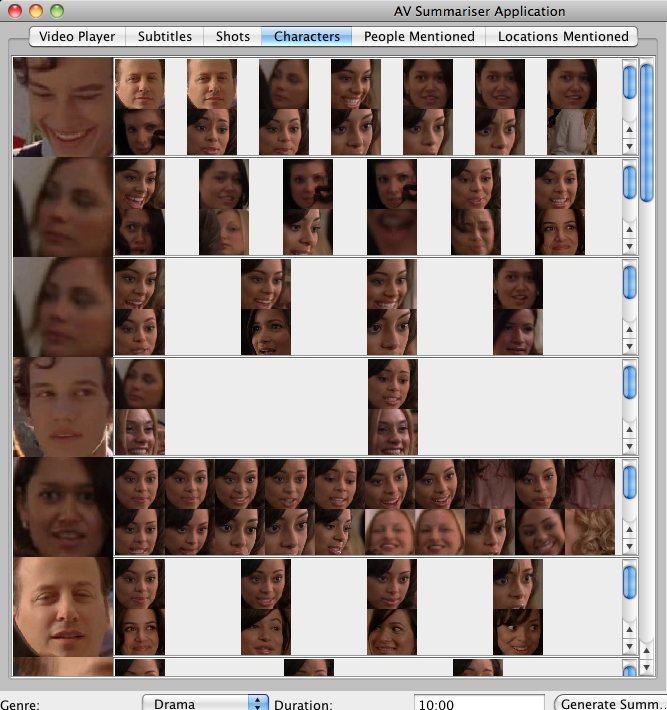
\includegraphics[trim = 0mm 0mm 0mm 0mm, clip,
 scale=0.4]{Images/Histogram.png}
  \caption{Histogram Comparison}
 \end{center}
\end{figure}

As shown above, this theory did not work well in practice and therefore the search for a better matching solution continued.

\newpage
\textbf{Pixel Comparison of the center and boundary areas of the detected faces:} This technique looked at the center square of a detected face, and the pixels in the center of each edge to try and find similarities. A screenshot showing the data gathered from this attempt is shown below:

\begin{figure}[ht]
\begin{center}
 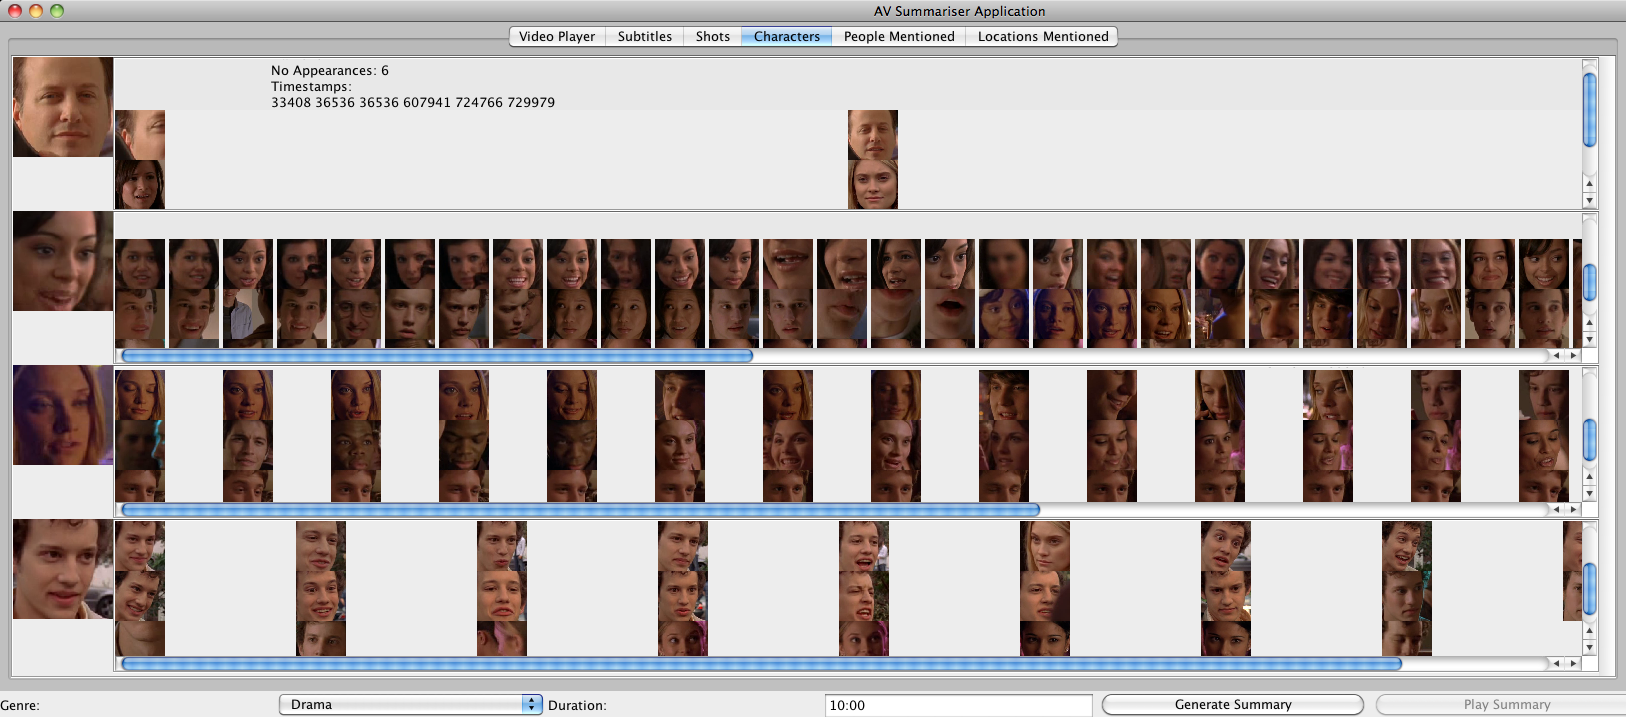
\includegraphics[trim = 0mm 0mm 0mm 0mm, clip,
 scale=0.26]{Images/PixelComparison.png}
  \caption{Pixel Comparison}
 \end{center}
\end{figure}

As with the previous attempt, it can be seen from the image above that this theory also didn't work well in practice. 

\newpage
\textbf{SIFT Comparison of Image Keypoints:} This technique used an aligner to line up the images and then extracted and compared the image 
keypoints. It was initially designed to draw the similar points between images, however in this method the number of matches were logged and if 
two images had over three matches (the logic being that such points as eyes, nose and mouth would be the type of keypoints) then a positive match was logged. Two 
screenshots showing some of the best examples of this technique in action are shown below:

\begin{figure}[h1]
\begin{minipage}[b]{0.5\linewidth}
 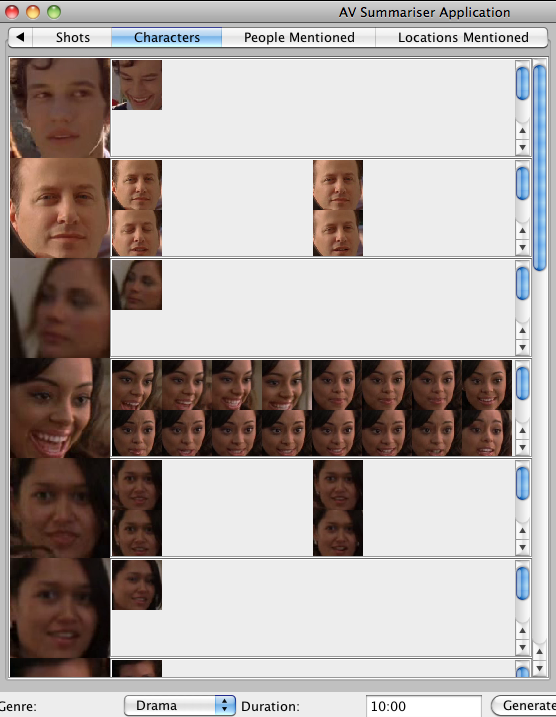
\includegraphics[trim = 0mm 0mm 0mm 0mm, clip,
 scale=0.38]{Images/SIFT.png}
  \caption{SIFT Comparison}
\end{minipage}
\hspace{0.5cm}
\begin{minipage}[b]{0.5\linewidth}
 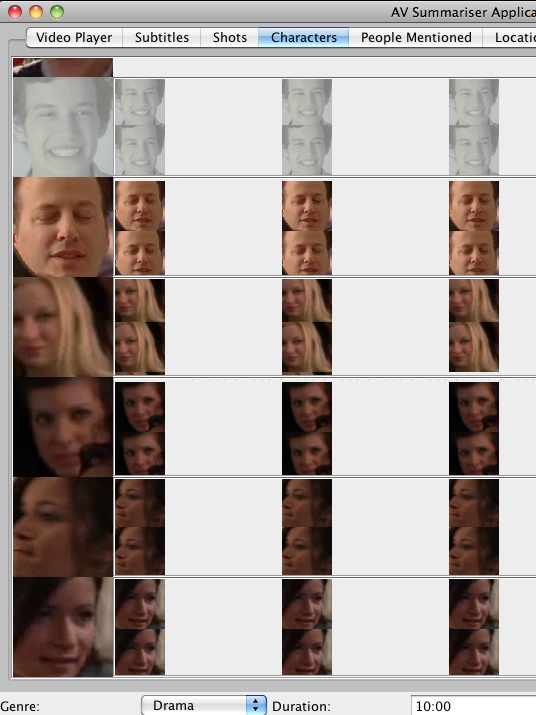
\includegraphics[trim = 0mm 0mm 0mm 0mm, clip,
 scale=0.38]{Images/SIFT2.png}
  \caption{SIFT Comparison}
\end{minipage}
\end{figure}

In conclusion to this section, the fourth technique as demonstrated above was chosen as the final clustering technique as even though it's good results are highly dependant on a well lit video where the faces can easily be extracted, it is still by far the most successful method attempted.

\newpage
\textbf{Face Matching}
\newline
The final step in this section was to match the characters to the actors playing them. The TVDB link as discussed previously (see Section \ref{sec:TVDB}) provides Objects with images of all the main characters of each 
series complete with actor names. For each character that contained enough matches, their images were added to a naive bayes recogniser and that 
was trained to recognise the different characters. Once this had been done, each series main character was tried against this to find the best match, 
if a match was positive then that character would be renamed by their actor name. This section could not be laboriously tested as it involved finishing 
the video in terms of facial recognition which meant that with the memory problems (discussed in a following section) it could only be tested on very short video clips. Nonetheless some experimentation was performed and below is a screenshot showing this:

\begin{figure}[ht]
\begin{center}
 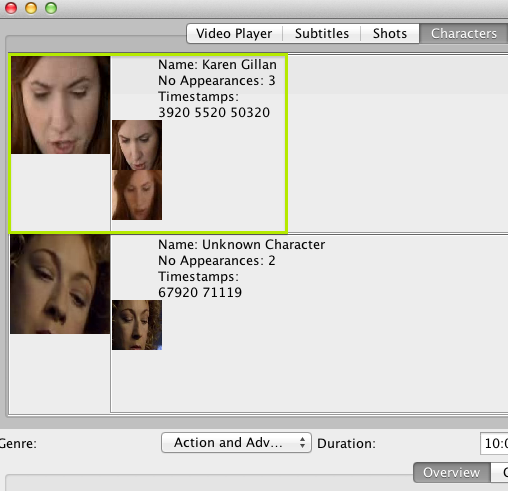
\includegraphics[trim = 0mm 0mm 0mm 0mm, clip,
 scale=0.64]{Images/ActorMatching.png}
  \caption{Pixel Comparison}
 \end{center}
\end{figure}

As you can see from the picture above, it has had problems with identifying non-faces still so only one of the characters has enough images to be matched with an actor. However, the actor in this case has been correctly identified.

\newpage

\subsubsection{Class Diagram}
The structure of the classes used within the package are shown in the class diagram below and detailed in further detail below.

\begin{figure}[h1]
\begin{center}
 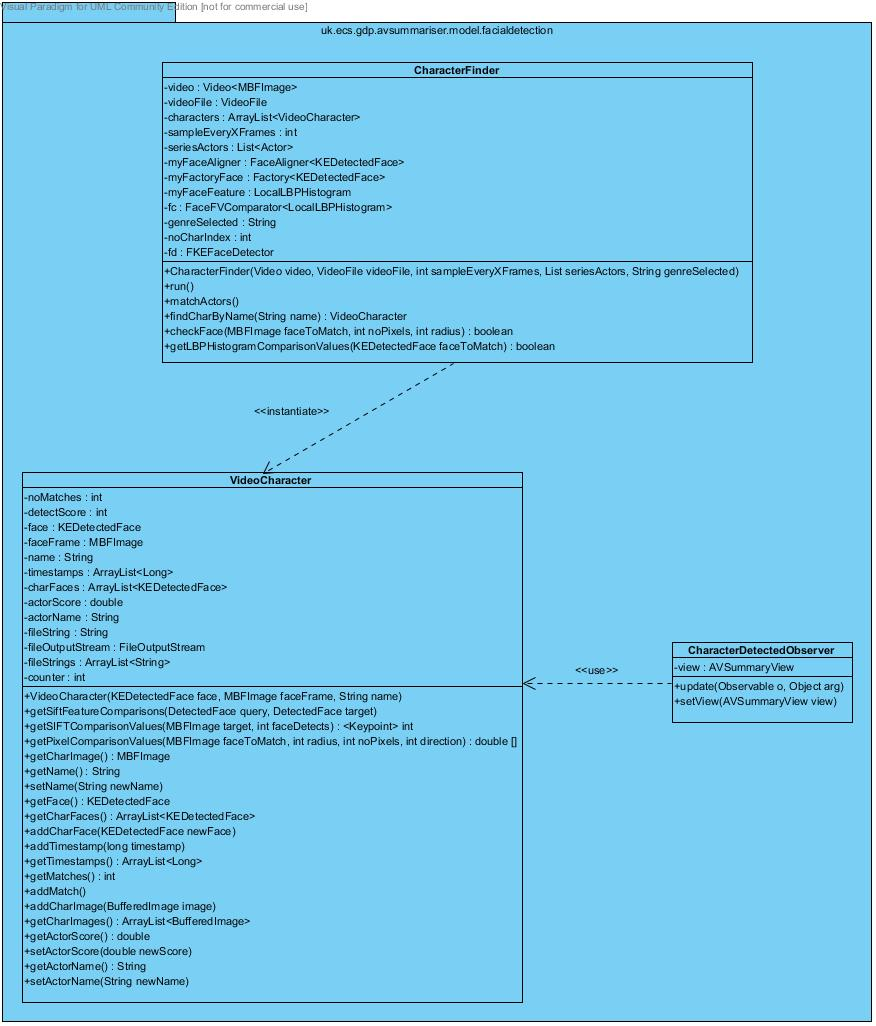
\includegraphics[trim = 0mm 0mm 0mm 0mm, clip,
 scale=0.5]{Images/facialdetection_package_class_diagram.jpg}
  \caption{Facial Detection Package Class Diagram}
 \label{fig:DrWhoFD}
 \end{center}
\end{figure}

\newpage
\subsubsection{Process Diagram}
A diagram of how the different modules chain together to produce the facial detection and recognition is given in the following Figure:

\begin{figure}[h1]
\begin{center}
 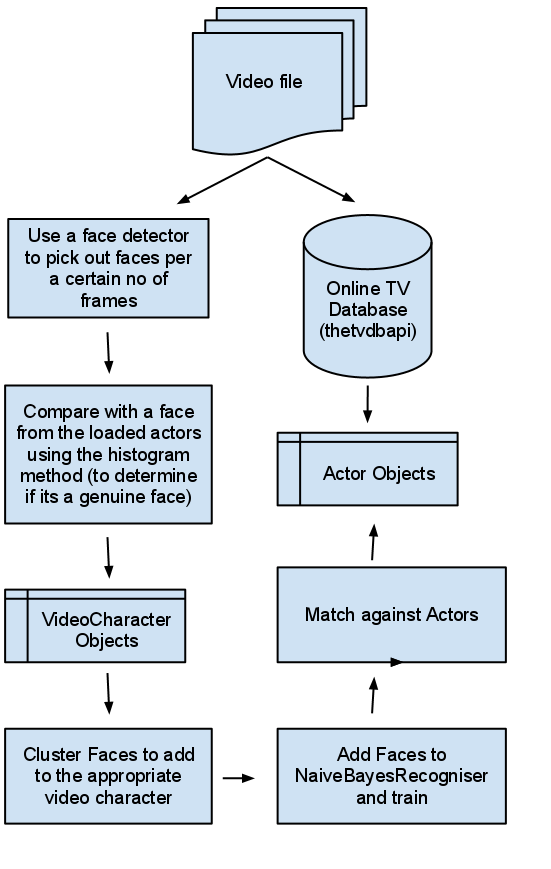
\includegraphics[trim = 0mm 0mm 0mm 0mm, clip,
 scale=0.5]{Images/FacialRecognitionProcess.png}
  \caption{Facial DetectionProcess Diagram}
 \label{fig:DrWhoFD}
 \end{center}
\end{figure}

\subsubsection{VideoCharacter}
A class which represents each individual character found in the video. It stores their image, timestamps and all the matching images that 
correspond to those timestamps. Due to memory problems instead of storing each matching image, these images are serialised and stored in a 
object output stream with references to the temporary files so that they can be read in at the appropriate time. Each VideoCharacter is displayed as an 
image in the Character panel and when clicked on expands to display the images of the character's appearances in the video and the timestamp links that jump to that area of the video. 

\subsubsection{CharacterFinder}
\label{sec:CharacterFinder}
A class which is responsible for locating, saving and matching the characters. It works in the following way:
\begin{itemize}
	\item{\textbf{Stage 1} - Lists all the identified faces in each frame that is looked at}
	\item{\textbf{Stage 2} - Performs the advanced face detection analysis on them to assess likliehood of being a face}
	\item{\textbf{Stage 3} - Checks to see if there are any existing characters that they are likely to match, if so that face is added to that character and its match value is incremented, if not a new character is created with that image}
	\item{\textbf{Stage 4} - Once it has clustered the characters, it puts them into a face recogniser and trains it}
	\item{\textbf{Stage 5} - That face recogniser then runs all the main characters produced by the TV Database (see Section \ref{sec:TVDB}) 
	to see if any of those characters are a likely match and if so renames them accordingly}.
\end{itemize}

\subsubsection{CharacterDetectedObserver}
This class implements the Observer interface and works with the Character Finder in Section \ref{sec:CharacterFinder} to draw the images of the detected characters in the character panel of the user interface. When the Character Finder wants to display a character it just has to notify the observer and that will call the appropriate methods in the GUI to draw their picture and show the corresponding information such as timestamps. 

\newpage 
\subsubsection{User Walkthrough}
Despite the facial recognition section not being added into the final summary production, characters can still be found within the team's system. The two screenshots below demonstrate the functionality and how it may be used: 

\textbf{Step 1:} Add a video, select it and add the series information (as shown in Section \ref{sec:TVDB}). Select ``Find Characters" and move to the Character Tab. Once a face is displayed, select it to see corresponding matches and timestamps. 
\begin{figure}[ht]
\begin{center}
 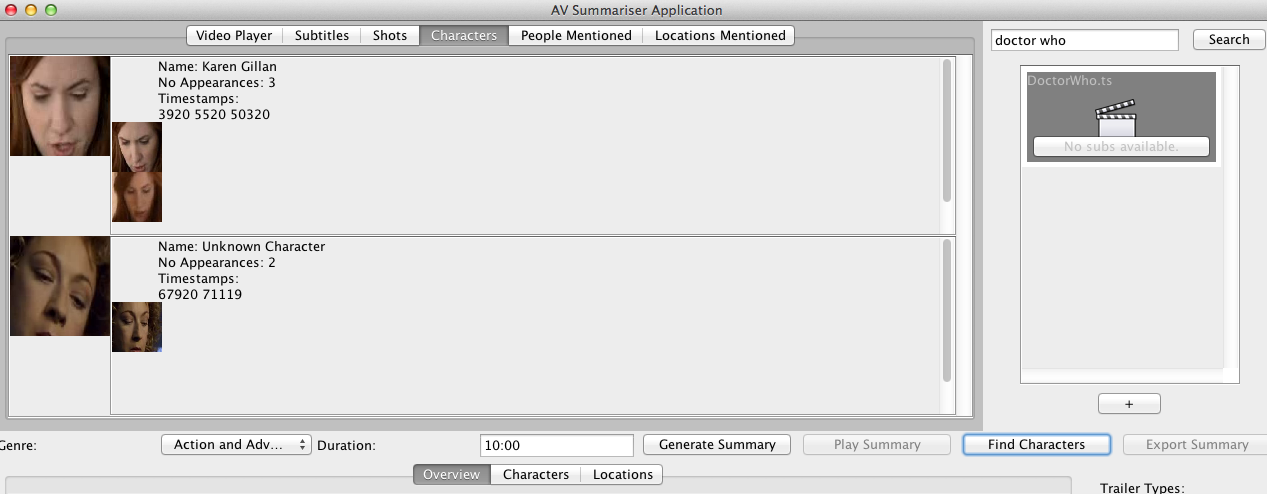
\includegraphics[scale=0.31]{Images/FaceWalkthrough1.png}
  \caption{Selecting a video and series and viewing the faces as they are detected}
 \end{center}
\end{figure}

\textbf{Step 2:} Wait for it to finish, and then click on the faces once again to see if they have been matched with an actor. 
\begin{figure}[ht]
\begin{center}
 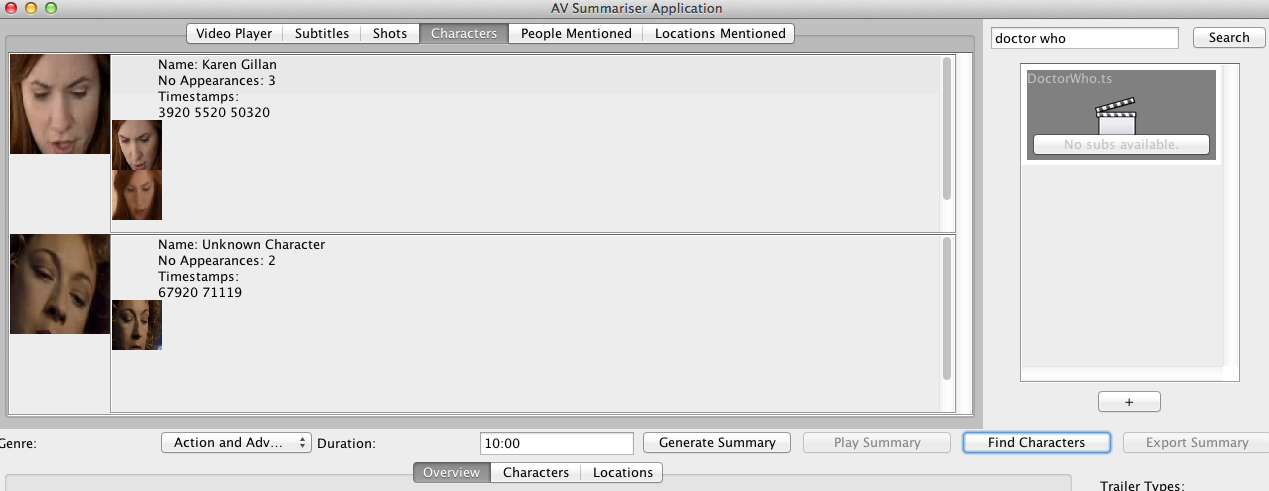
\includegraphics[scale=0.31]{Images/FaceWalkthrough2.png}
  \caption{Viewing all the detected faces and their matched actors}
 \end{center}
\end{figure}

\newpage

\subsection{Video Segmentation} 
\label{sec:VideoSeg}
\subsubsection{Introduction}
A key goal of the project was to enable segmenting a video in a way which appreciated
how the video was made up. Some of the modules of the system will give a specific point
in time (a timestamp) which represents something interesting, however this is not as useful
when considering how the information should be passed back to the user.

A video is made up of shots which are then grouped into scenes. A scene is a series of
shots in one location. An editor will use a variety of different shots, depending on the impressions that they wish to convey to the viewer. The lengths of shots or the density of shots can be used in a particular sequence to make inferences about what is happening in the video. For example, many varied short shots may represent an action sequence, or lengthy shots may be long shots where the film maker is setting the scene and showing little detail. 

Furthermore, looking at the video shot data alongside the subtitle information, the shots may correlate with the different actors who speak. 
This could suggest a director is using over shoulder shots in a conversation. This information, particularly when combined with other data about the video, can be a powerful tool in summarising video content.

\subsubsection{Software Implementation}
The OpenIMAJ library on which the team is basing the project, has a video shot detector. This
uses histogram differences to find the changes in shots.

\begin{figure}[h1]
\begin{center}
 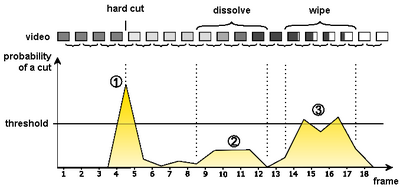
\includegraphics[trim = 0mm 0mm 0mm 0mm, clip,
 scale=1.4]{Images/Cut_Detection_Diagram.png}
  \caption{Shot Cut detection}\label{fig:cutDetectionDiagram}
 \end{center}
\end{figure}

It is down to the team to set the threshold or the sensitivity of the detector. This was done by
simply watching the video and counting the frames, then checking to see if the shot processing
returned a similar number. Shot detection is a hard problem for a computer to solve,
it is relatively easy to fool the system into thinking that there is a shot change. For example in the screenshot below a man in a tunnel can be seen. 
The tunnel is unstable, so dirt is falling in front of the camera, which is detected as a large color change between frames so that a new shot is detected. This particular example could be addressed by reducing the sensitivity of the detector, but this is not always the case.

\begin{figure}[h1]
\begin{center}
 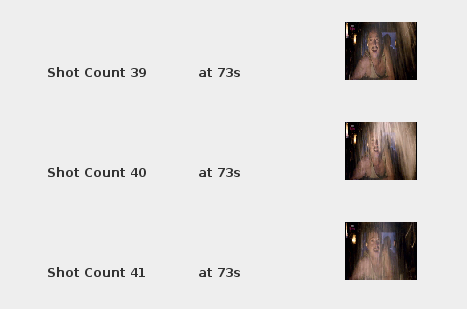
\includegraphics[trim = 0mm 0mm 0mm 0mm, clip,
 scale=1.2]{Images/shot-detection-incorrect-cut.png}
  \caption{Incorrect cut in shot detection  - threshold too low}\label{fig:incorrectCutShotDetection}
 \end{center}
\end{figure}

Some events such as lighting in the video could not be ignored, so a few errors are likely to
exist. On the whole however, errors are quite minimal and spread across a series the results
are not noticeable. A listener is then attached to the video to fire an event when a
shot change is detected. This provides a key frame which is scaled down to a thumbnail
and keep in order to represent the shot to the user.

In the application, when the user clicks on a video, shot detection is started and the frame
thumbnail representing each shot is output to the GUI, with a count of the number of
shots and the time of the shot. This is for demonstration/informational purposes. 
The shot detection is threaded and shot detection can take place on multiple
videos at any one time.

When the user chooses to generate a summary the system will ensure that the shots have
been detected for all loaded videos. The data is then made available to the video summary
builder.

\newpage 
\subsubsection{User Walkthrough}
Below are two screenshots indicating how to initiate shot detection:

\textbf{Step 1:} Add video and select it. 
\begin{figure}[ht]
\begin{center}
 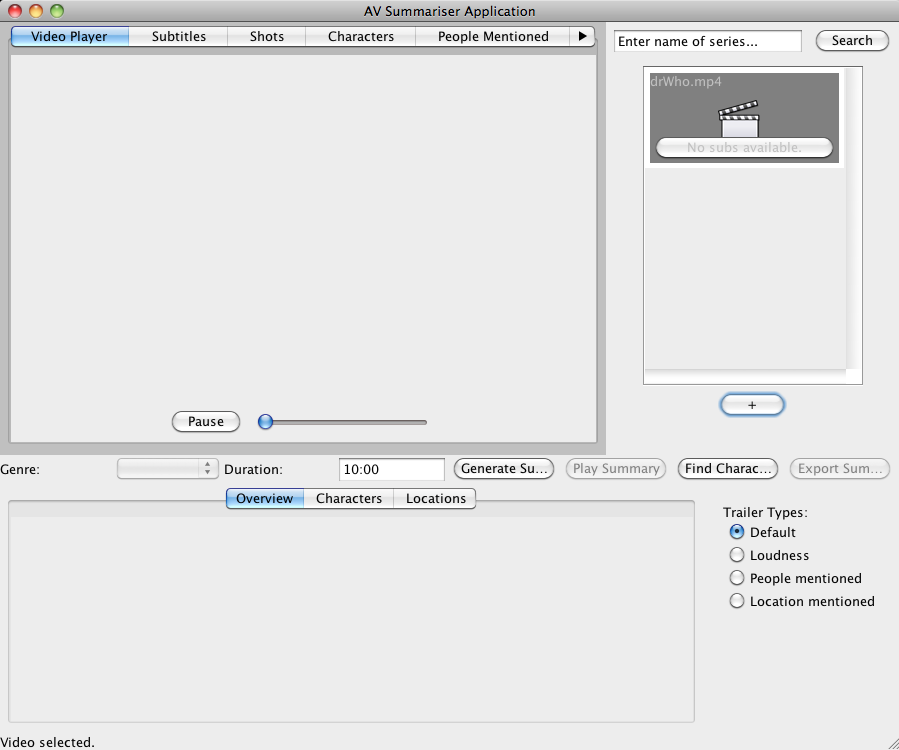
\includegraphics[scale=0.31]{Images/ShotDetectionWalkthrough1.png}
  \caption{Adding a video and selecting it}
 \end{center}
\end{figure}

\textbf{Step 2:} Press ``Generate Summary" and the different shots will appear in the Shot Tab. 
\begin{figure}[ht]
\begin{center}
 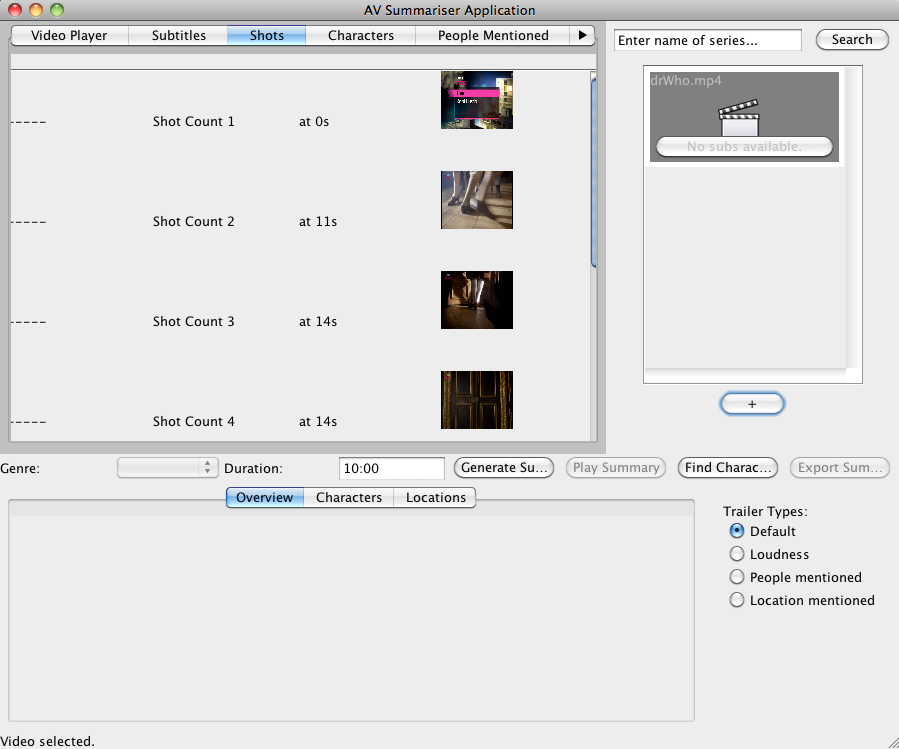
\includegraphics[scale=0.31]{Images/ShotDetectionWalkthrough2.png}
  \caption{Viewing the Shot Detection Output}
 \end{center}
\end{figure}

\newpage

\subsection{Summarisation}
\label{sec:Summarisation}

\textbf{Package: uk.ecs.gdp.avsummariser.model.summary}

This package contains all the Java code that produces the summary using all the data produced from the previous modules. This package has the following purposes:
\begin{itemize}
	\item{Using all the information produced by the system (excluding Frequency Detection and Face Detection which has been explained previously) and the user's metrics such as: Genre selected, Trailer duration, Trailer type.To produce a Summary object containing all the merged data and a trailer.}
	\item{Using a produced Summary object export all the data produced into three files which are:}
	\begin{itemize}
		\item{A trailer for the television series.}
		\item{A XML file called ``summary\_xml" which contains all the summary information such as metrics used, Series object information, Actor object information and all people mentioned with timestamps.}
		\item{A XML file called ``data\_xml" which for each video file loaded contains:}
		\begin{itemize}
			\item{The subtitle file associated with that video file.}
			\item{All the data that the different modules produced for that video and subtitle file.}
		\end{itemize}
	\end{itemize}
\end{itemize}

\subsubsection{Process Diagram}
A diagram of how the different modules chain together to produce the summary is given below:

\begin{figure}[h1]
\begin{center}
 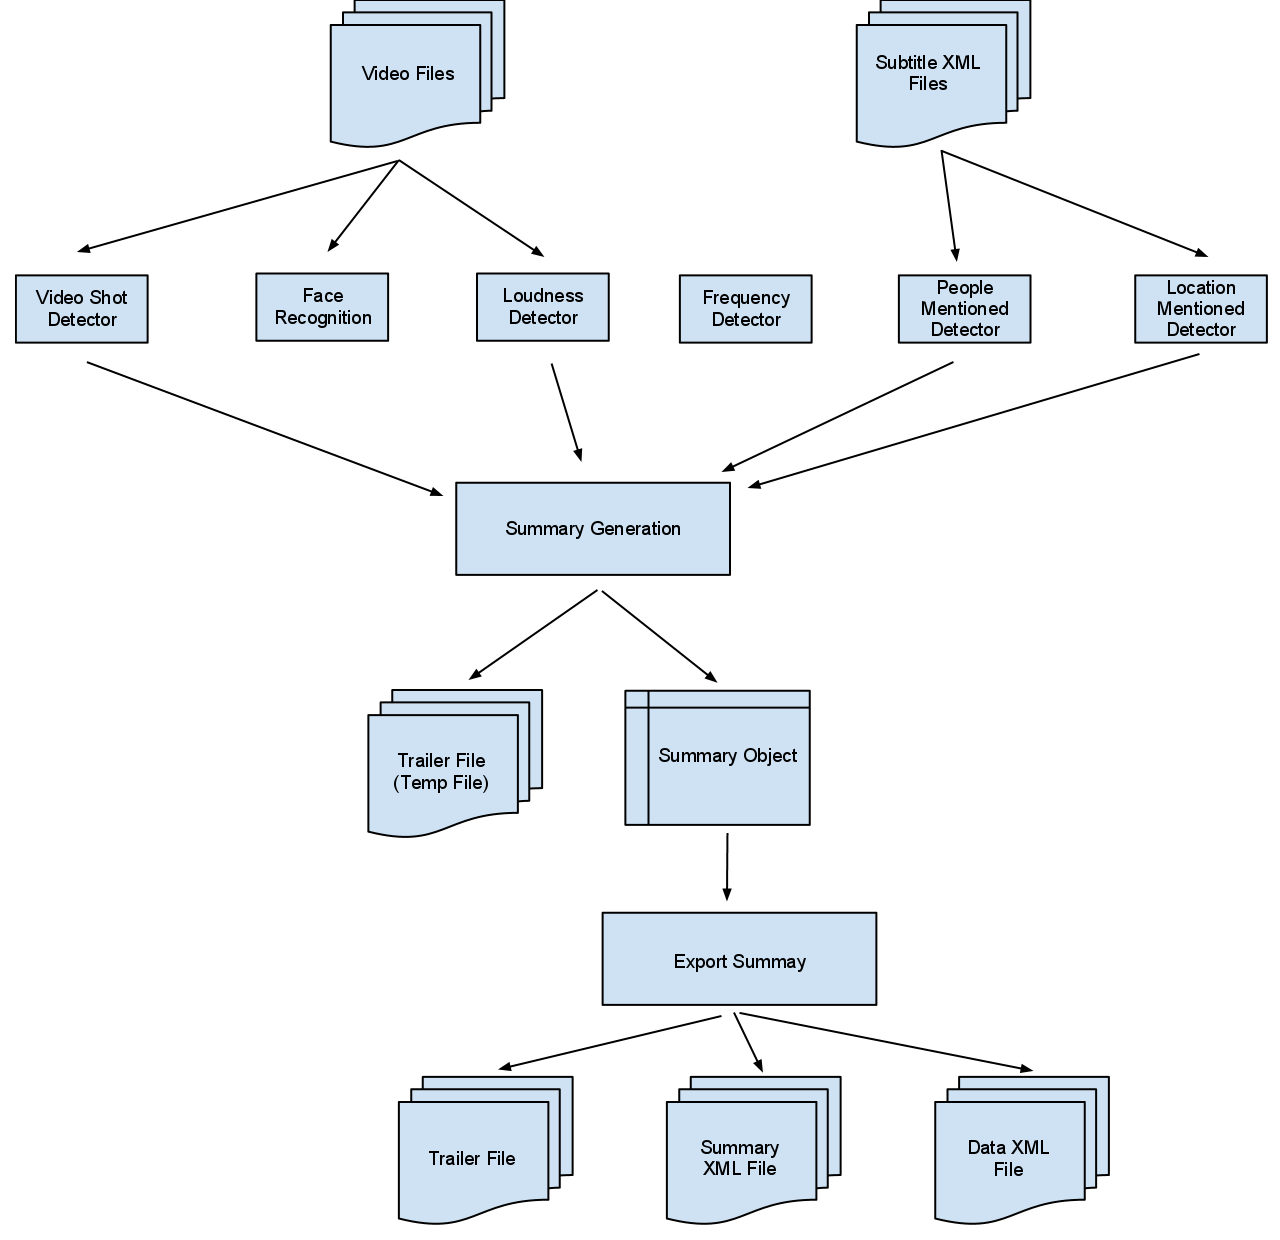
\includegraphics[trim = 0mm 0mm 0mm 0mm, clip,
 scale=0.2]{Images/SummaryProductionProcess.png}
  \caption{Summary Process Diagram}
 \end{center}
\end{figure}

\newpage
\subsubsection{Class Diagram}
The structure of the classes used within this package are shown in the class diagram below and detailed in further detail below.

\begin{figure}[ht]
\begin{center}
 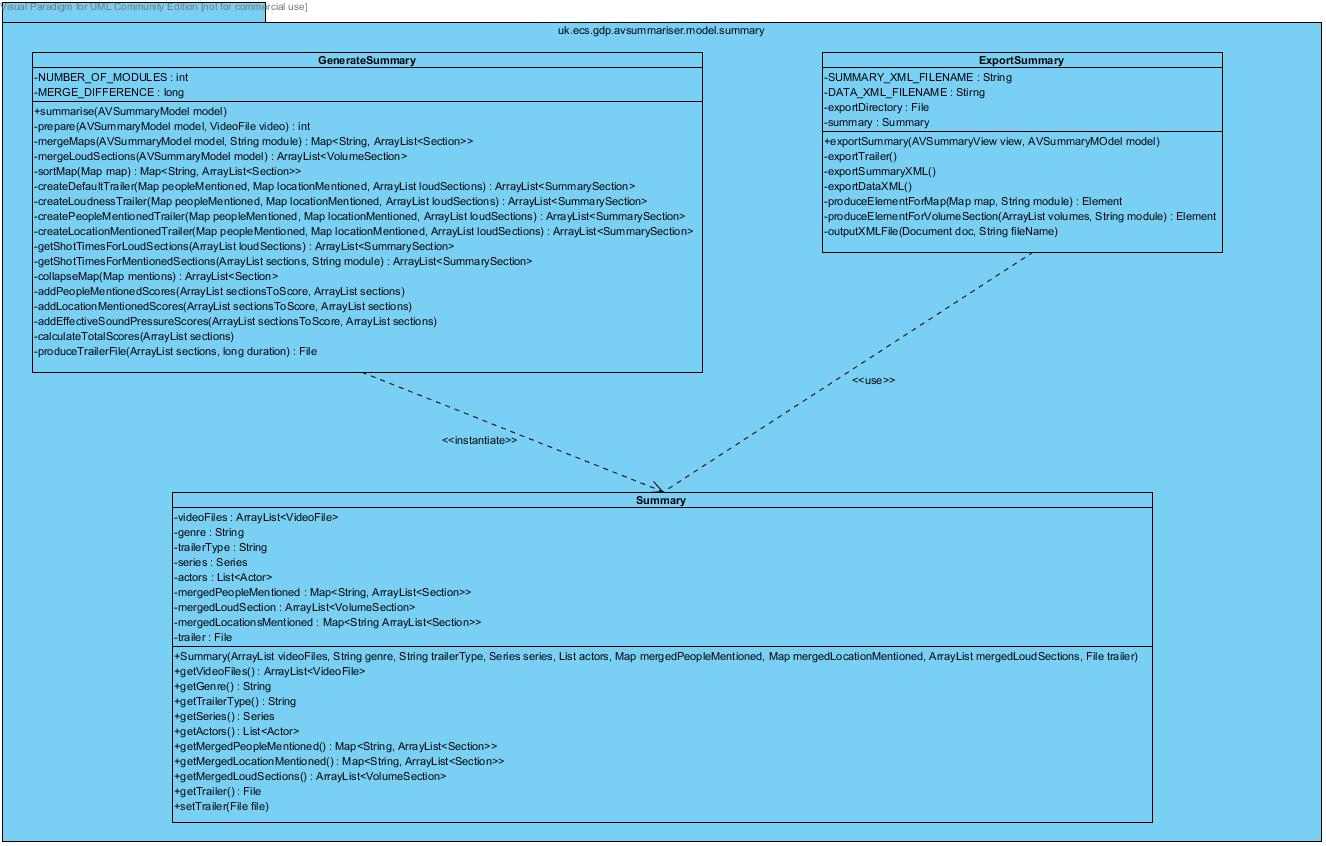
\includegraphics[trim = 0mm 0mm 0mm 0mm, clip,
 scale=0.33]{Images/summary_package_class_diagram.jpg}
  \caption{Summary Package Class Diagram}
 \end{center}
\end{figure}

\subsubsection{Summary}
This class is a container object for all data that is gathered and produced for all the files that are loaded into the system

\subsubsection{GenerateSummary}
A static class which produces the Summary Object and video summary. How this is done depends on what metrics the user selects, which is discussed in the following stages:

\textbf{Stage 1:} Firstly, the system checks whether the different modules which are currently used have been ran and completed for each video file input. These various modules are:
\begin{itemize}
	\item{Video shot detection.}
	\item{Person name detection.}
	\item{Location name detection.}
	\item{Loudness detection.}
\end{itemize}

If not then they are ran and the system waits until all modules have completed for all video files. 

\textbf{Stage 2:} Next the following sets of data for each video are merged together:
\begin{itemize}
	\item{People names mentioned.}
	\item{Location names mentioned.}
	\item{Loud sections.}
\end{itemize}
into a container for each.

\textbf{Stage 3:} Now the system chooses what video shots to use in the trailer. This depends on the trailer type the user selected currently these are the options:
\begin{itemize}
	\item{Default.}
	\item{Loudness.}
	\item{People Mentioned.}
	\item{Locations mentioned.}
\end{itemize}
Which option the user selects becomes the priority in choosing video shots. This is how generally the video shots are chosen with further details underneath about what is chosen for each trailer type.

\textbf{Stage 3A:} An initial set of video shots is selected. This is done using either an ArrayList of Section or VolumeSection 
Objects. These are mapped to the VideoShots which contain them and are around three seconds in length.
\begin{itemize}
	\item{Default: VolumeSection Objects for loud sections used.}
	\item{Loudness: VolumeSection Objects for loud sections used.}
	\item{People Mentioned: Section Objects for people mentioned used.}
	\item{Locations Mentioned: Section Objects for locations mentioned used.}
\end{itemize}

\textbf{Stage 3B:} Due to this rounding there may be repeats, overlapping or unable to be merged with the VideoShots Objects. 
These conditions are then checked for and the VideoShots are merged based on these conditions and the scores are adjusted as appropiate. This is done to produce an ArrayList of SummarySection Objects (these contain scores for each type of module used) and at the moment will contain only one type of score.

\begin{itemize}
	\item{Default : ESP scores.}
	\item{Loudness : ESP scores.}
	\item{People Mentioned :  People mentioned scores.}
	\item{Locations Mentioned : Location's mentioned scores.}
\end{itemize}

\textbf{Stage 3C:} Other score types are added to the SummarySection Object. For People and Location scores the scores are calculated as follows 
by doing the following for each Section Object and adding the individual scores together:

\begin{itemize}
	\item{If the start and end time of the Section Object is fully contained in this SummarySection then add a one.}
	\item{Else if it starts and doesn’t finish in the Section or vice versa then add 0.5.}
	\item{Else if not contained add zero.}
\end{itemize}

Whereas for ESP scores it is the averge of the ESP score for the SummarySection Object plus the ESP of the current VolumeSection Object multiplied by x (Where x is either 1, 0.5 or 0). 
\begin{itemize}
	\item{Default: People mentioned and Location's mentioned scores.}
	\item{Loudness: People mentioned and Location's mentioned scores.}
	\item{People Mentioned: ESP and Location's mentioned scores.}
	\item{Locations Mentioned: ESP and People mentioned scores.}
\end{itemize}

\textbf{Stage 3D:} The total score is calculated for all SummarySection Objects (people names mentioned score plus Location names mentioned score).

\textbf{Stage 3E:} The SummarySection Object list is sorted in descending order according the trailer type chosen.
\begin{itemize}
	\item{Default: Total score then ESP score.}
	\item{Loudness: ESP score then Total score.}
	\item{People Mentioned: People score then Total score.}
	\item{Locations Mentioned: Location score then Total score.}
\end{itemize}

\textbf{Stage 4:} Using the priority sorted SummarySection ArrayList produced, the SummarySection Objects to go in the trailer are chosen while the total time is less than or equal to the target duration the user wanted.

\textbf{Stage 5:}  SummarySection Objects are sorted back into video filename order and then time order, before creating a summary by splitting up the separate videos as required for the desired shots and are finally concatenated together to produce a summary.

\textbf{Stage 6:} Finally a Summary Object is produced containing the summary produced, all important merged summary data and individual data produced for each video.

\subsubsection{ExportSummary}
A static class presents a file chooser to the user to choose where to export the Summary object and all its content to. Once selected the trailer file is moved from the TEMP directory to where the user selected and two XML files are produced using JDOM\cite{jdom} containing the information detailed earlier.

\newpage
\subsubsection{User Walkthrough}
Below are six screenshots indicating how to generate a summary and the information that becomes available once it has been created: 

\textbf{Step 1:} Load in videos, and subtitles (optional) and select ``Generate Summary":
\begin{figure}[h1]
\begin{center}
 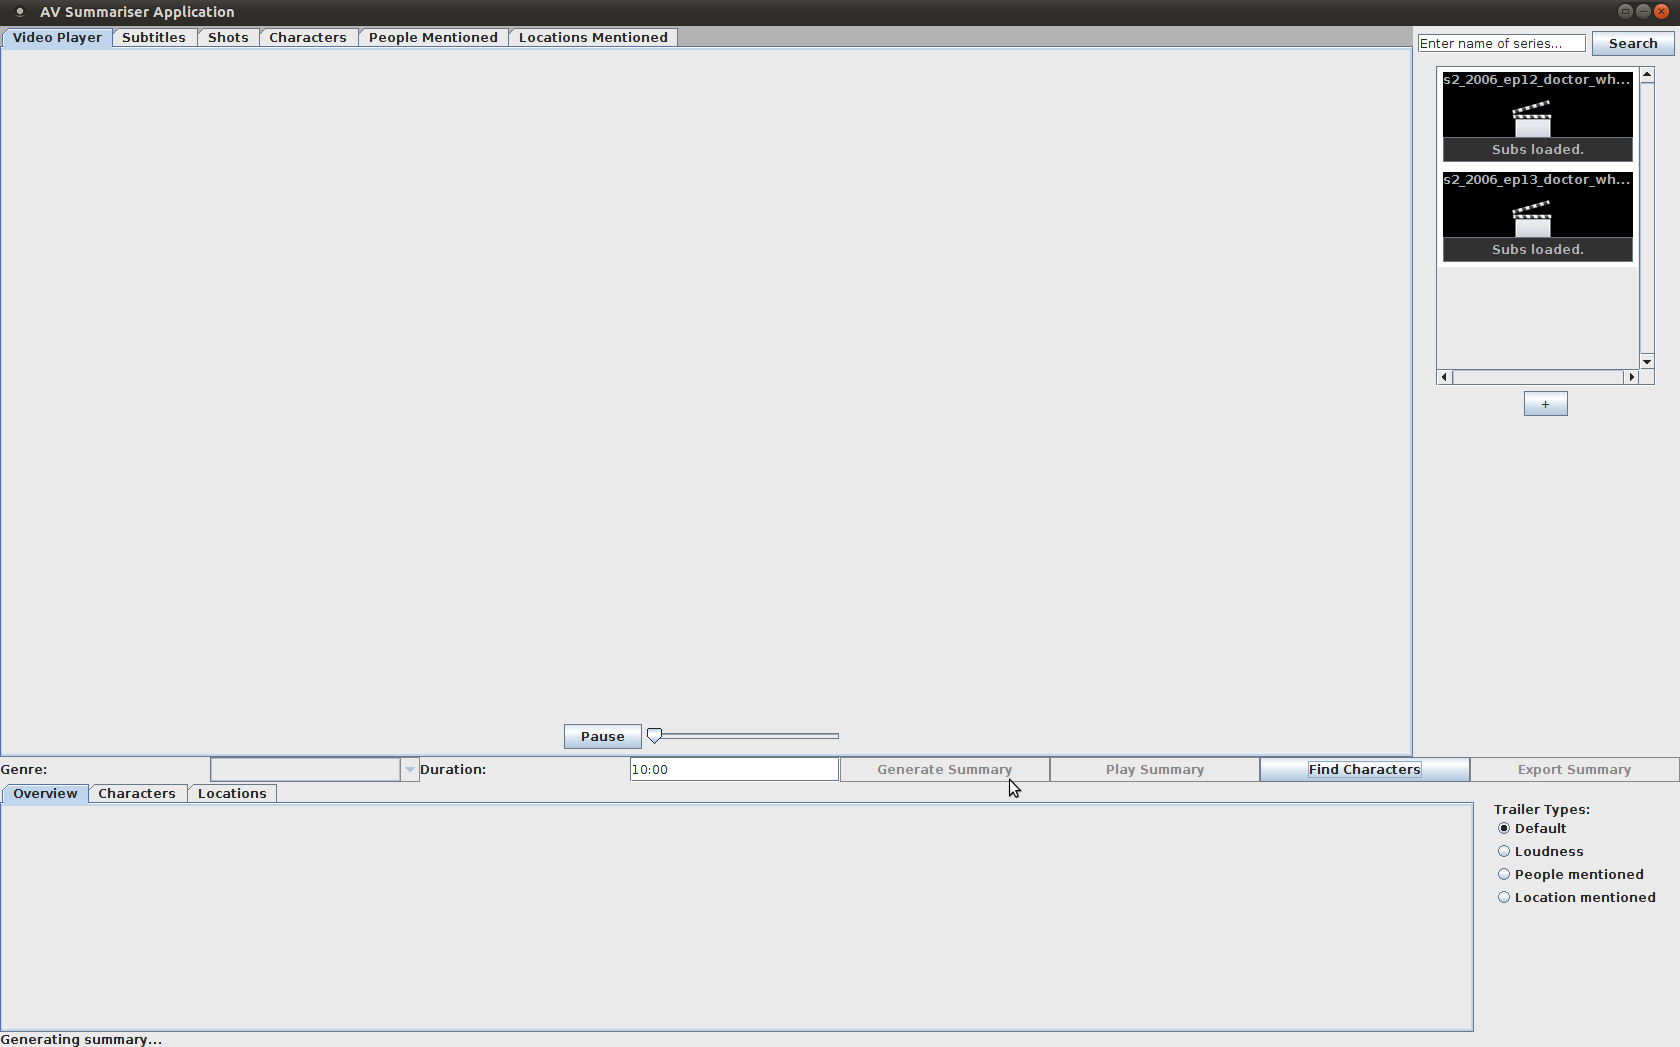
\includegraphics[trim = 0mm 0mm 0mm 0mm, clip,
 scale=0.22]{Images/01PressingGenerate.png}
  \caption{Pressing Generate Summary}
 \end{center}
\end{figure}

\textbf{Step 2:} Observe the Overview Tab to view the information loaded in from the TV Database \cite{tvdb}:
\begin{figure}[h1]
\begin{center}
 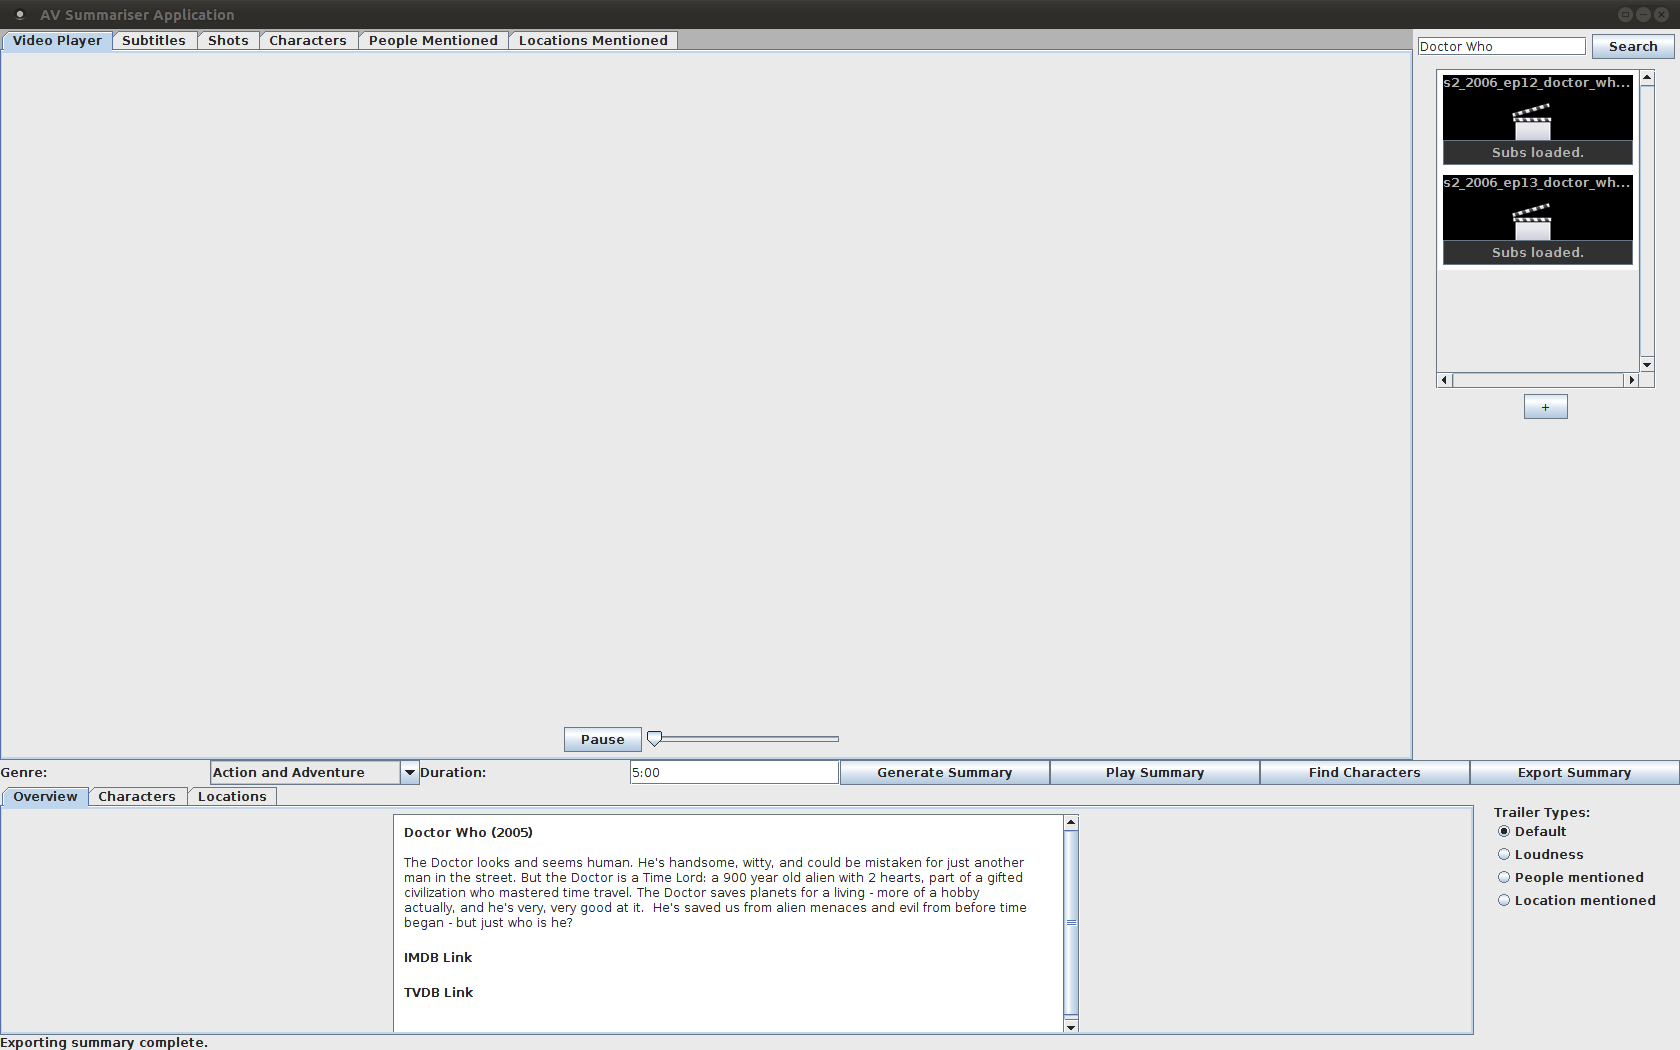
\includegraphics[trim = 0mm 0mm 0mm 0mm, clip,
 scale=0.22]{Images/02OverviewTab.png}
  \caption{The Overview Tab}
 \end{center}
\end{figure}

\newpage

\textbf{Step 3:} Observe the Character Tab to view the information generated by the summary. 
\begin{figure}[h1]
\begin{center}
 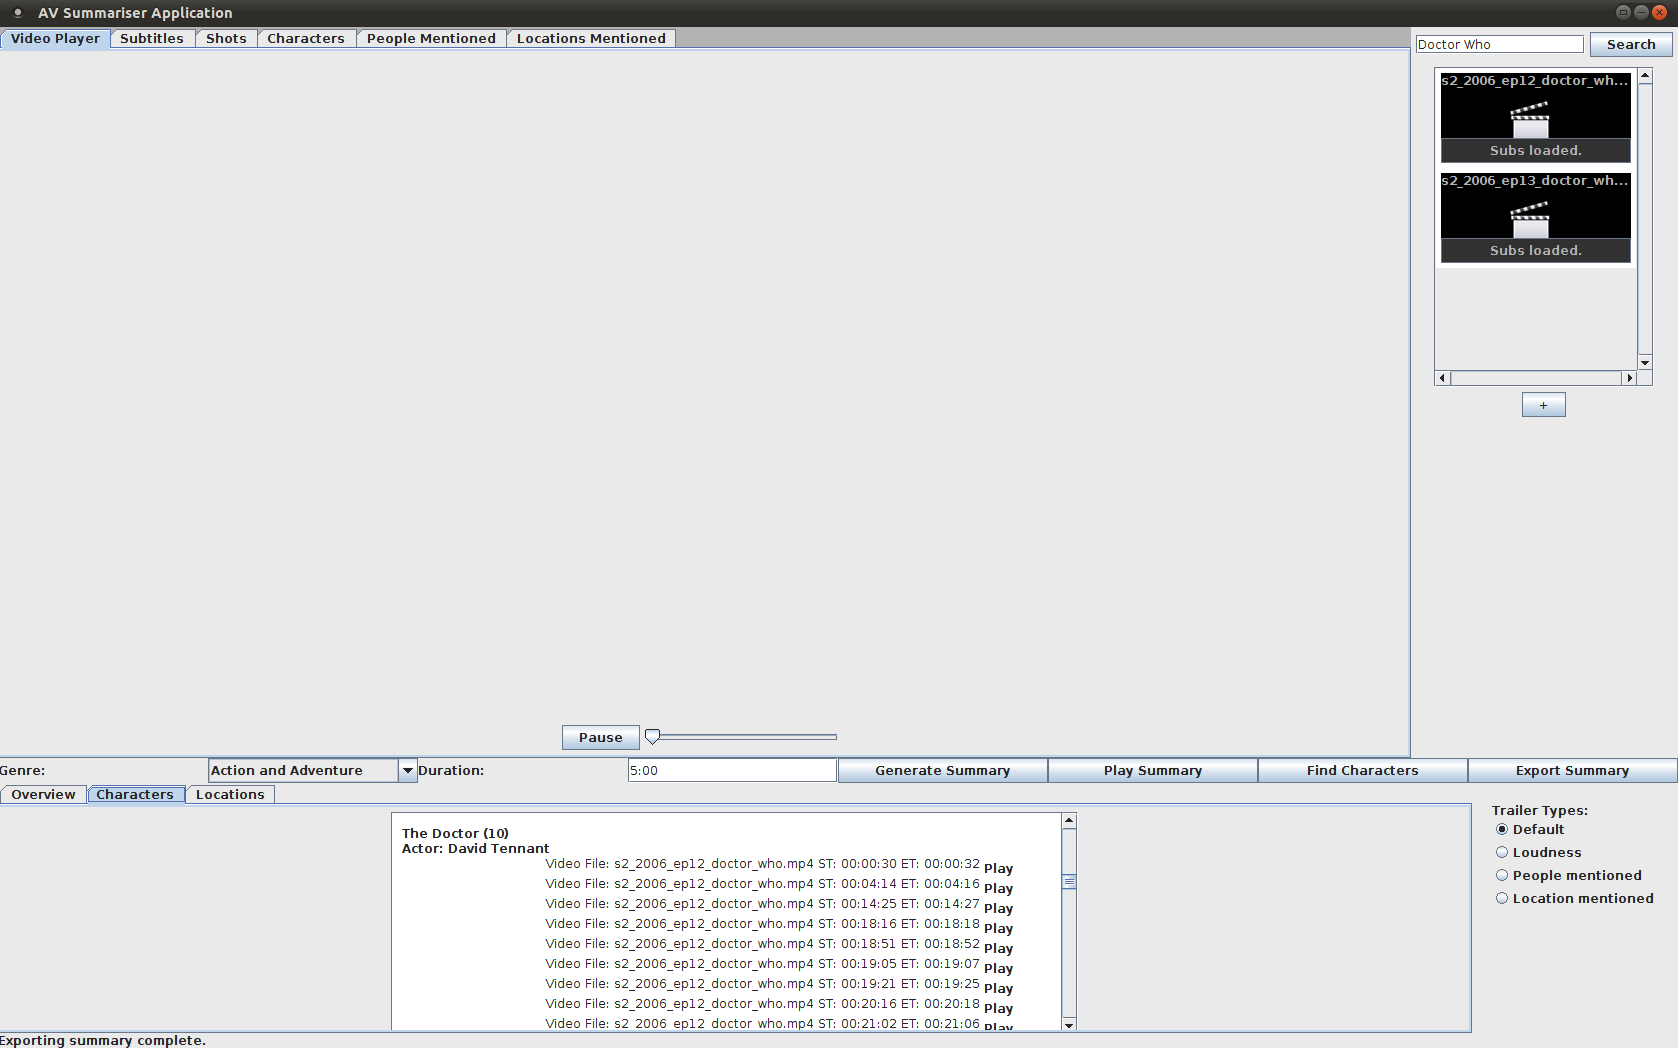
\includegraphics[trim = 0mm 0mm 0mm 0mm, clip,
 scale=0.22]{Images/03CharactersTab.png}
  \caption{The Character Tab}
 \end{center}
\end{figure}

\textbf{Step 4:} Observe the Location Tab to view the information generated by the summary. 
\begin{figure}[h1]
\begin{center}
 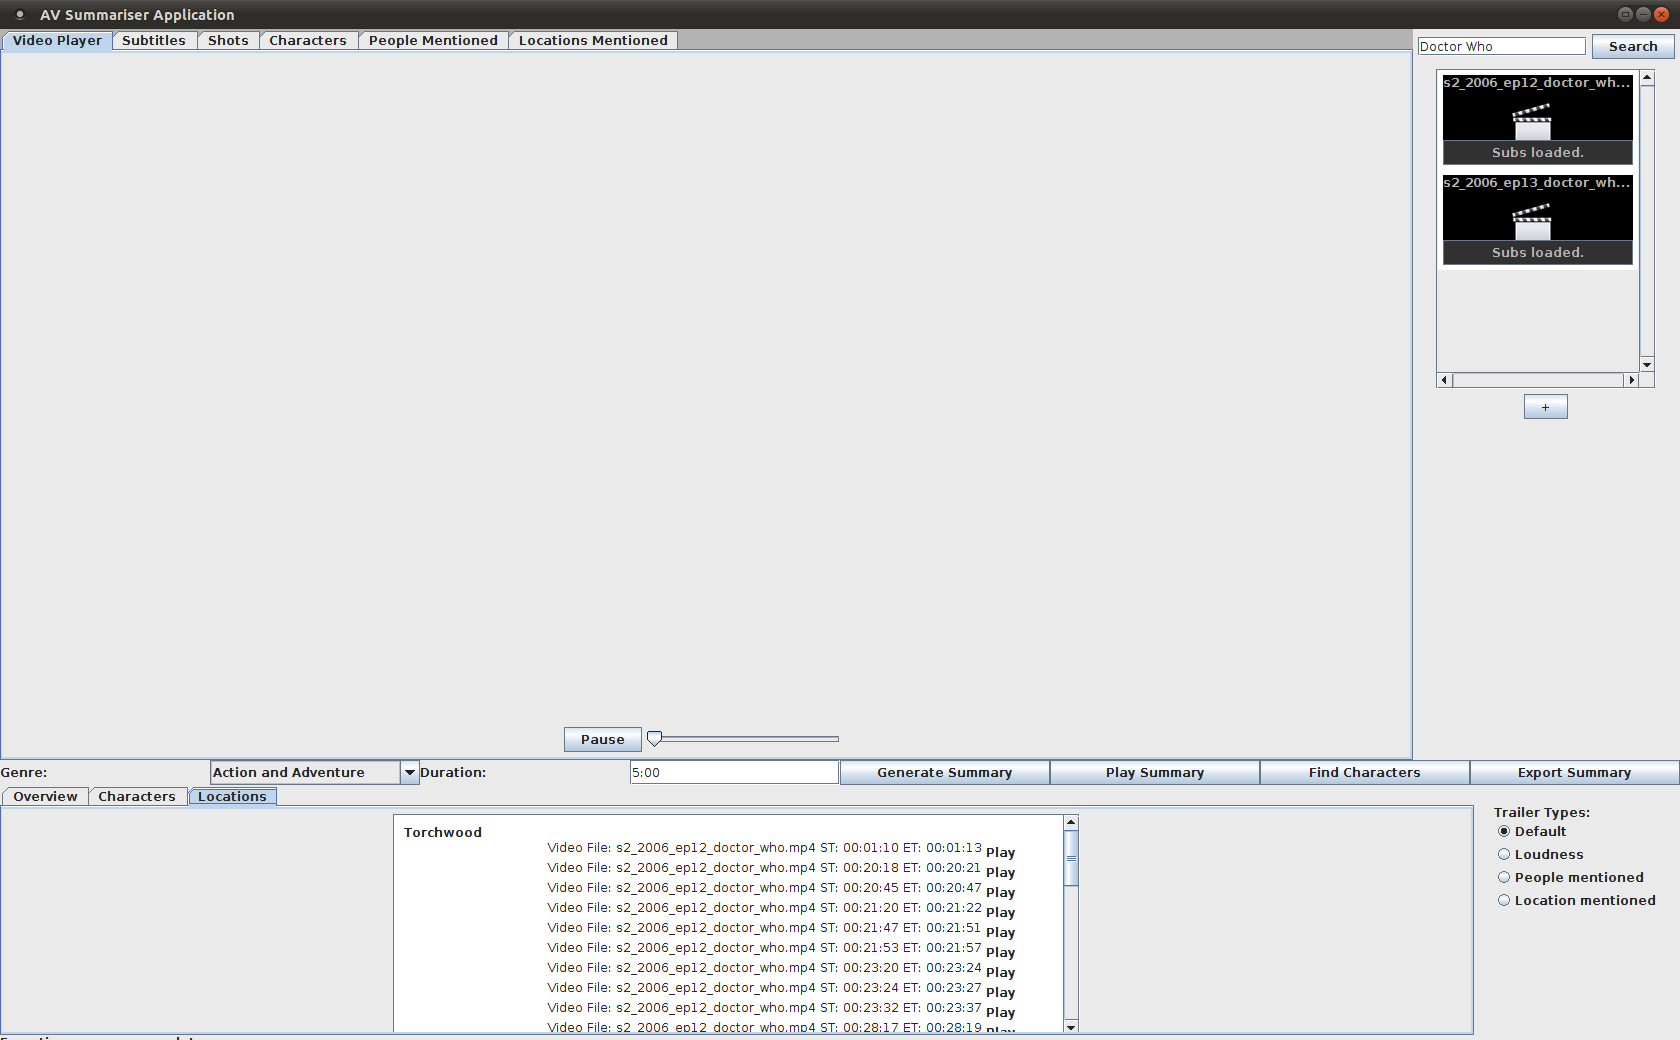
\includegraphics[trim = 0mm 0mm 0mm 0mm, clip,
 scale=0.2]{Images/04locationsTab.png}
  \caption{The Locations Tab}
 \end{center}
\end{figure}

\newpage

\textbf{Step 5:} Click on the ``Play" button of a location timestamp to seek to that scene in the video. 
\begin{figure}[h1]
\begin{center}
 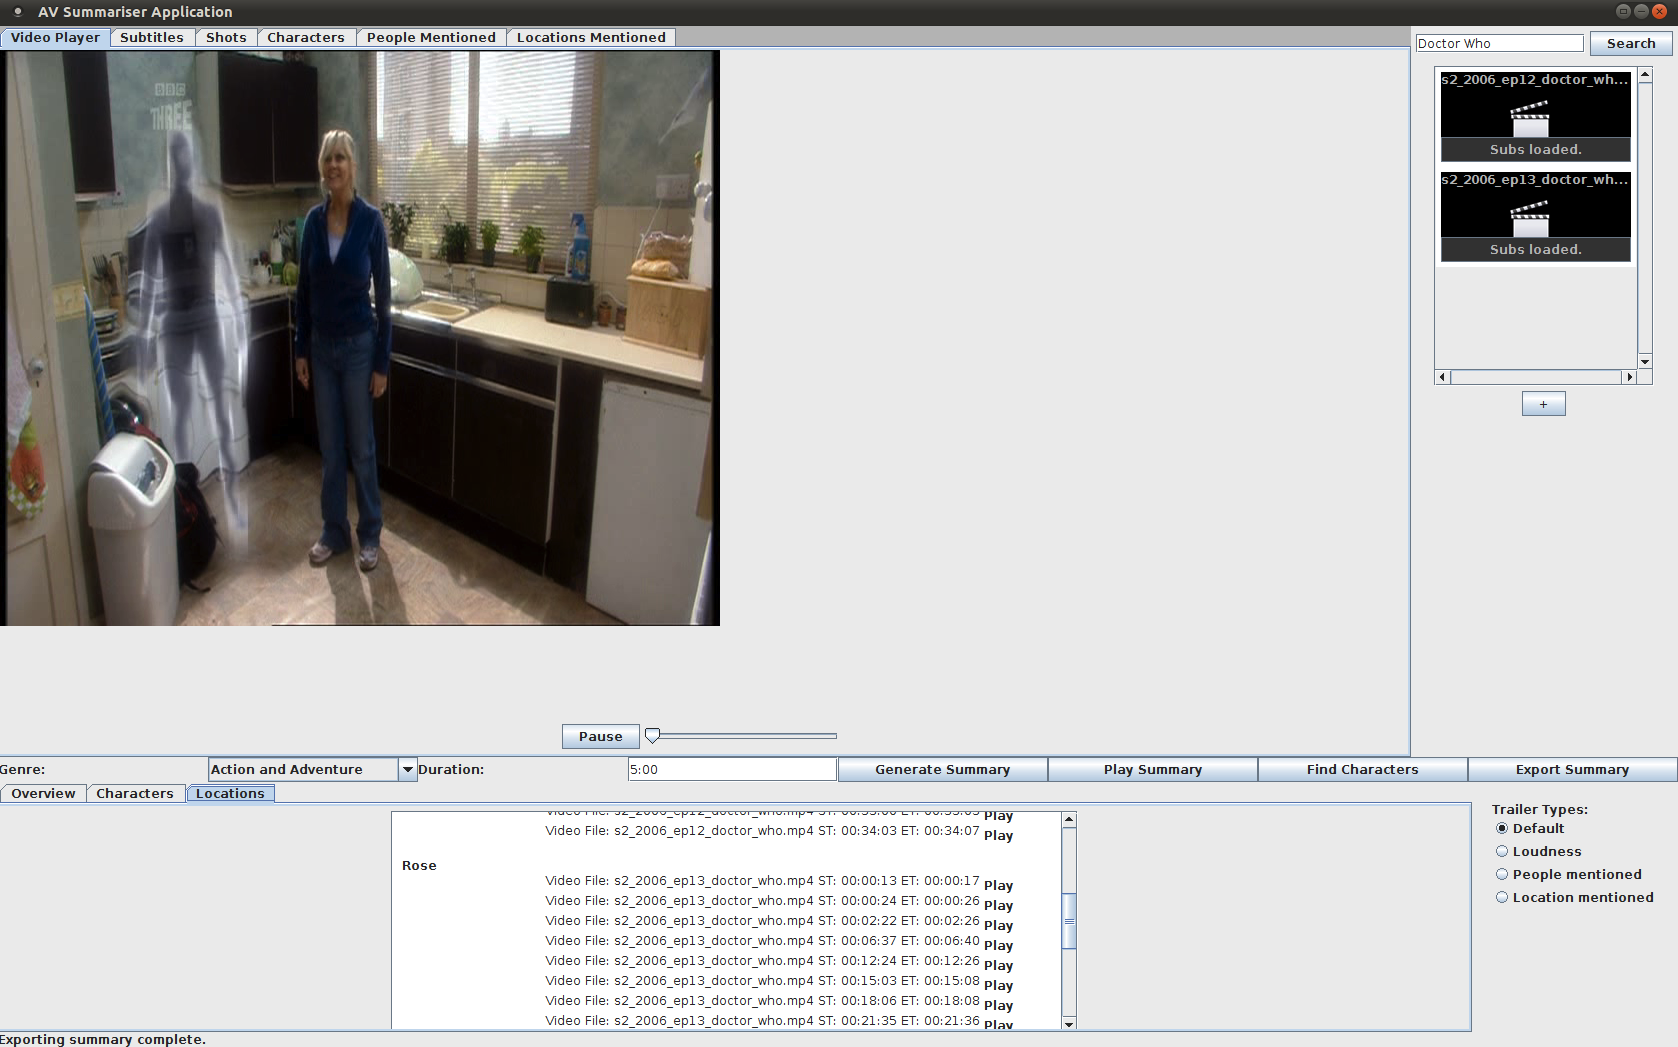
\includegraphics[trim = 0mm 0mm 0mm 0mm, clip,
 scale=0.22]{Images/05locations-Skipto.png}
  \caption{Using the Locations data to skip to that scene in the video}
 \end{center}
\end{figure}

\textbf{Step 6:} Click on the ``Export Summary" button and select where to export it to. 
\begin{figure}[h1]
\begin{center}
 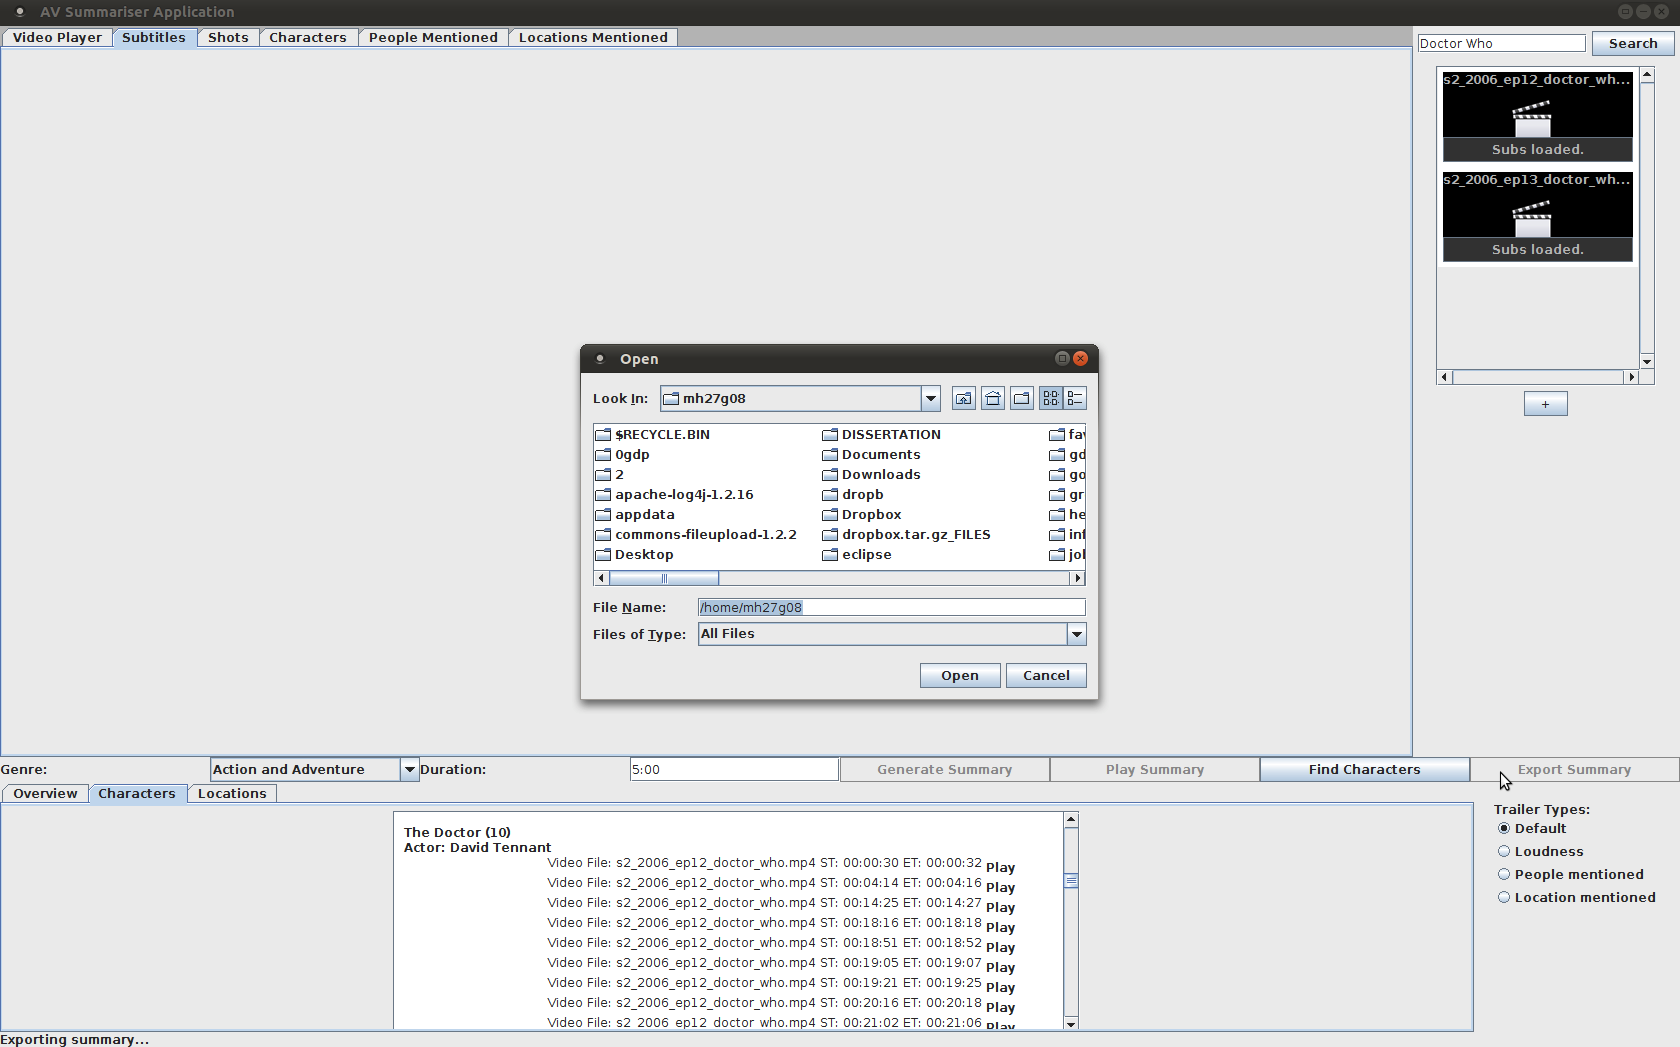
\includegraphics[trim = 0mm 0mm 0mm 0mm, clip,
 scale=0.22]{Images/06Exporting.png}
  \caption{Exporting the Summary}
 \end{center}
\end{figure}

\newpage
\subsection{User Interface}

Packages: 
\begin{itemize}
	\item{\textbf{uk.ecs.gdp.avsummariser.view}}
	\item{\textbf{uk.ecs.gdp.avsummariser.view.viewbrowser}}
	\item{\textbf{uk.ecs.gdp.avsummariser.view.pot}}
\end{itemize}
The packages listed above contain all the View code which constructs the user interface; a screenshot of how the user interface looks is given below.

\begin{figure}[h1]
\begin{center}
 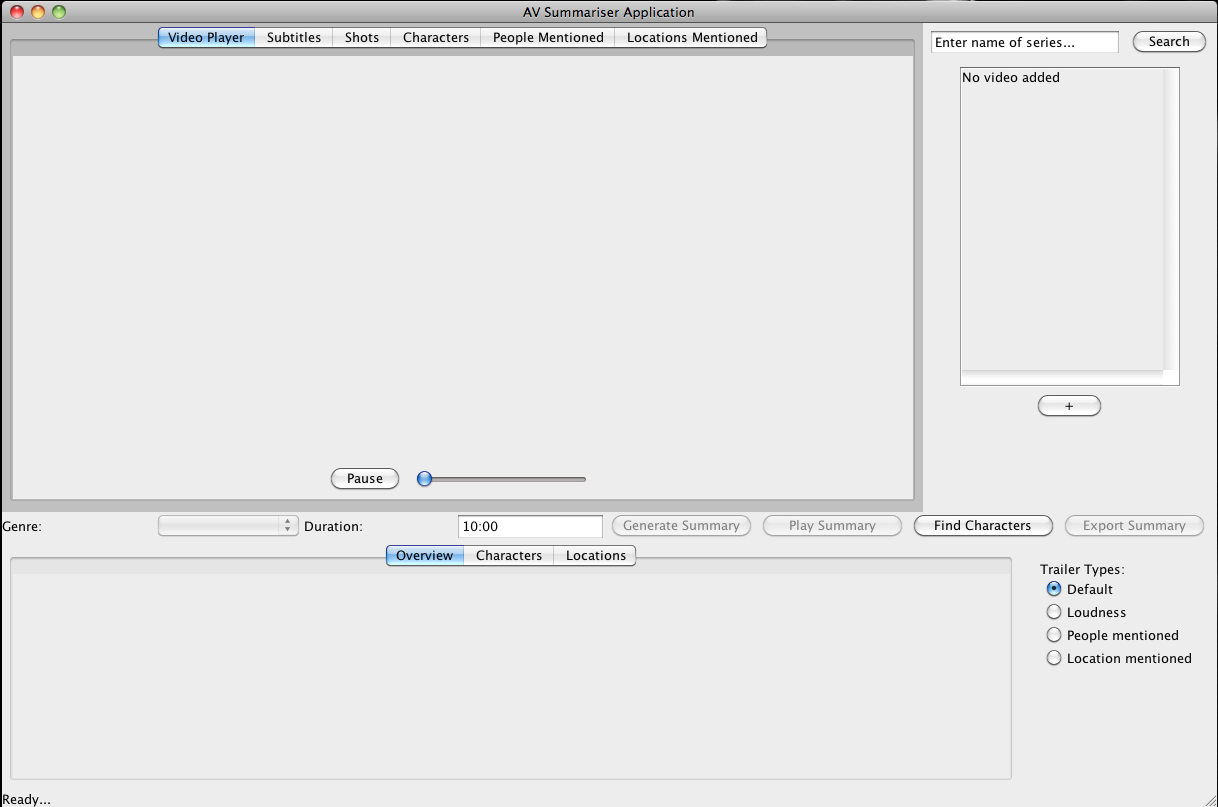
\includegraphics[trim = 0mm 0mm 0mm 0mm, clip,
 scale=0.35]{Images/UIScreenshot.png}
  \caption{User Interface Screenshot}
 \end{center}
\end{figure}

All the classes within these packages are either subclasses of JFrame, JTabbedPane or JPanel and come together to allow the user to view all output of system and control how the processing is done by entering/selecting summary metrics such as trailer target duration, the television series they wish to use, etc.
